 %%%%%%%%%%%%%%%%%%%%%%%%%%%%%%%%%%%%%%%%%
% Stylish Article
% LaTeX Template
% Version 2.2 (2020-10-22)
%
% This template has been downloaded from:
% http://www.LaTeXTemplates.com
%
% Original author:
% Mathias Legrand (legrand.mathias@gmail.com)
% With extensive modifications by:
% Vel (vel@latextemplates.com)
%
% License:
% CC BY-NC-SA 3.0 (http://creativecommons.org/licenses/by-nc-sa/3.0/)
%
%%%%%%%%%%%%%%%%%%%%%%%%%%%%%%%%%%%%%%%%%

%----------------------------------------------------------------------------------------
%	PACKAGES AND OTHER DOCUMENT CONFIGURATIONS
%----------------------------------------------------------------------------------------

\documentclass[10pt]{SelfArx} % Document font size and equations flushed left

\usepackage[english]{babel} % Specify a different language here - english by default
\usepackage{pgfgantt}

\usepackage{lipsum} % Required to insert dummy text. To be removed otherwise

\usepackage{booktabs}


%----------------------------------------------------------------------------------------
%	COLUMNS
%----------------------------------------------------------------------------------------

\setlength{\columnsep}{0.55cm} % Distance between the two columns of text
\setlength{\fboxrule}{0.75pt} % Width of the border around the abstract

%----------------------------------------------------------------------------------------
%	COLORS
%----------------------------------------------------------------------------------------

\definecolor{color1}{RGB}{0,0,90} % Color of the article title and sections
\definecolor{color2}{RGB}{0,20,20} % Color of the boxes behind the abstract and headings

%----------------------------------------------------------------------------------------
%	HYPERLINKS
%----------------------------------------------------------------------------------------

\usepackage{hyperref} % Required for hyperlinks

\usepackage{float}
\usepackage{makecell}
\hypersetup{
	hidelinks,
	colorlinks,
	breaklinks=true,
	urlcolor=color2,
	citecolor=color1,
	linkcolor=color1,
	bookmarksopen=false,
	pdftitle={Title},
	pdfauthor={Author},
}
\usepackage{multicol}
\usepackage{float}

%----------------------------------------------------------------------------------------
%	ARTICLE INFORMATION
%----------------------------------------------------------------------------------------

\JournalInfo{Laboratory of biological data mining} % Journal information
\Archive{Project report} % Additional notes (e.g. copyright, DOI, review/research article)

\PaperTitle{Medulloblastoma: Human Specific Genes Contributions} % Article title

\Authors{Sara Baldinelli\textsuperscript{1}, Letizia De Pietri\textsuperscript{1}, Gaia Faggin\textsuperscript{1}, Huyen Pham\textsuperscript{1}, Roan Spadazzi\textsuperscript{1}} % Authors
\affiliation{\textsuperscript{1}\textit{University of Trento, Trento 38123, Italy}} % Author affiliation

\Keywords{} % Keywords - if you don't want any simply remove all the text between the curly brackets
\newcommand{\keywordname}{Keywords} % Defines the keywords heading name

%----------------------------------------------------------------------------------------
%	ABSTRACT
%----------------------------------------------------------------------------------------

\Abstract{Medulloblastoma (MB) is the most prevalent malignant brain tumor in childhood. It poses a significant health challenge and impacts children at a rate tenfold higher than adults. The disease is molecularly heterogeneous, with distinct subgroups (WNT, SHH, GP3, and GP4) exhibiting variations in cytogenetics, mutational profiles, and gene expression signatures, shaping treatment strategies and outcomes. Since the disease origins are primarily genomic alterations, we aim to investigate if the MB driving genes are also Human Specific Genes (HSGs). As HSGs are unique to humans, they often underpin distinctive traits that evolved recently or undergo significant changes. As a result, they often play critical roles in brain functions, immune systems, and metabolic processes. Our research seeks to identify MB HSGs, their function and their potential for being bio-markers and drug targets. To this aim, we retrieved both a cases and a control MB datasets, we pre-processed them and we analyzed the outputs. In particular, we carried out network and functional analyses on sets of genes that were found to be differentially expressed between MB cases and controls or between one of the four MB subgroups and controls. The results of the analyses confirmed the robustness of our datasets, showing patterns expected in the MB gene environment. Also, we identified a set of genes that can be considered for further studies as they were found to be particularly significant in MB development.}
%----------------------------------------------------------------------------------------

\begin{document}

\maketitle % Output the title and abstract box
%\tableofcontents % Output the contents section

%\thispagestyle{empty} % Removes page numbering from the first page

%----------------------------------------------------------------------------------------
%	ARTICLE CONTENTS
%----------------------------------------------------------------------------------------

\section*{Introduction}\label{sec:introduction}
Medulloblastoma (MB) stands as the most prevalent malignant brain tumor in childhood, constituting roughly 20\% of pediatric central nervous system tumors \cite{kumar2017challenges}, and impacting children at a rate tenfold higher than adults \cite{carta2020cancer}. This condition is categorized into distinct molecular subgroups: WNT, Sonic Hedgehog (SHH), Group 3 (GP3) and Group 4 (GP4) (\textbf{Table \ref{tbl:subtypes}}). These subgroups exhibit striking differences in cytogenetics, mutational profiles, and gene expression signatures, all of which significantly influence the treatment strategies and outcomes \cite{chen2022molecular}.\\
Given its prevalence in childhood, MB's origins cannot be attributed to environmental or age-related factors. Instead, it is primary driven by genomic alterations.
Previous studies showed that the least to most common sub-groups are: WNT, SHH, Group 3 and Group 4. Respectively, they have survival rates of: $\sim$95\%, $\sim$60-80\%, $\sim$50\% and, $\sim$75\% \cite{northcott2012medulloblastomics, hovestadt2020medulloblastomics}. 

\begin{table}[h!]
  \centering
    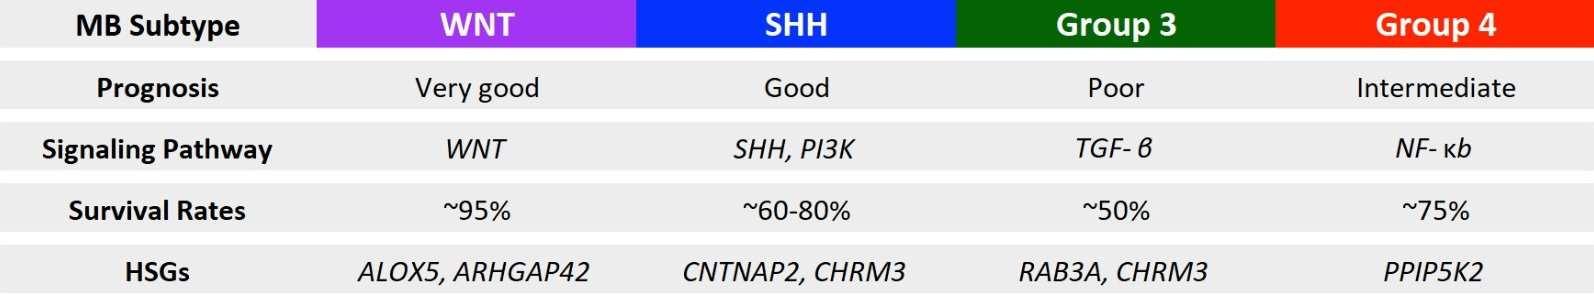
\includegraphics[width=1\textwidth]{project-report/figures/subtypes.jpeg}
    \caption{Table describing the main features of the four different subtypes of MB. The last row highlights the HSG we found, at the end of this study, to be related to each subtype.}
   \label{tbl:subtypes}
\end{table}

Currently, an insufficiently accurate disease risk stratification does not allow for therapies that are specific to standard or high-risk patients. Identifying potential biomarkers specific to each of the four sub-groups and associating them to a specific risk-ratio could introduce the application of more personalized therapies.\\
A way to narrow down the set of genes to investigate, is to consider the set of Human Specific Genes (HSGs) since a substantial portion of them plays a critical role in brain functions, alongside their roles in the immune system and metabolic processes \cite{bitar2019genes}.
HSGs are genes that are unique to the human species and have no direct counterparts in the genome of other closely related species, such as our primate relatives. These genes are often considered to be responsible for traits or functions that are distinctive to humans; they may have evolved relatively recently in the human lineage or have undergone significant changes that make them distinct from the genes found in other species. Identification and study of HSGs could provide insight into what sets humans apart from other species. \\ 
Consequently, in our project we will investigate the contribution of HSGs with respect to non-HSGs in the context of this disease.
More specifically, our efforts are directed towards identifying HSGs that may contribute to the development of MB. \\ 
To this purpose, we retrieved case and control datasets respectively from GSE155446 \cite{riemondy2022neoplastic} and GSE118068 \cite{vladoiu2019childhood}, pre-processed them and performed Differential Expression (DE) Analyses to obtain a list of statistically significant Differentially Expressed Genes (DEGs). \\
The so obtained list was expanded through causal relationships identified by the GENE@HOME project \cite{asnicar2015tn}. 
This was followed by network and functional analyses, which allowed us to highlight the potential role of the imputed genes. These analyses, together with a literature search, led us to formulate hypotheses about the role of HSGs in the context of MB. \\

\section{Materials}
\subsection{Datasets}\label{sec:Datasets}

\subsubsection{GSE155446}
Cohort GSE155446 \cite{riemondy2022neoplastic} represents a comprehensive exploration of cellular heterogeneity within $28$ childhood MB cases, classified into different subgroups, including $1$ WNT, $9$ SHH, $7$ GP3 and $11$ GP4 MB. \\
This study investigates cellular diversity in childhood MB using single-cell RNA sequencing, revealing distinct neoplastic cell sub-populations associated with mitotic, undifferentiated and neuronal profiles. \\
The cohort comprises a total of $39946$ cells and explores the expression patterns of $26841$ genes.

\subsubsection{GSE118068}\label{sec:GSE118068}
GSE118068 \cite{vladoiu2019childhood} cohort was chosen to serve as a reference point for normal cellular states. \\
This dataset comprises $9$ hindbrains gathered from diverse developmental stages, encompassing both embryonic and postnatal phases. Given that MB predominantly emerges in childhood, our emphasis was directed specifically towards the $4$ postnatal samples. By doing so we retrieved a total of $27997$ genes and $28210$ cells. 

\subsection{Homologous genes}\label{sec:homologous_genes}
We used a list of homologous genes downloaded from Ensembl (version 110) \cite{biomart_ensembl110} to identify matches between the two datasets under investigation. Employing this resource provided us with a reliable foundation for pinpointing meaningful homologous relationships.  

\subsection{Human Specific Genes}\label{sec:human_specific_genes}
A list of $856$ of HSGs was retrieved from the study conducted by Bitar et al \cite{bitar2019genes}. This comprehensive list was employed as a valuable reference for identifying HSGs within the broader set of genes after the DE analysis.

\subsection{FANTOM \& GENE@HOME}\label{sec:Fantom_dataset}
The GENE@HOME \cite{asnicar2015tn} initiative represents an implementation of the PC-IM algorithm, designed to enhance Gene Regulatory Networks (GRN). The project utilizes gene causal relations extracted from the FANTOM dataset \cite{fantom5} to unravel the complexities of these regulatory networks.
Through its utilization we aim to expand the set of MB HSGs and identify causal relations to be further investigated during our analysis.


\subsection{STRING}
For an initial functional investigation the STRING database \cite{szklarczyk2019string} with default parameters was used. STRING compiles data from various origins, incorporating experimental findings, computational predictions, and publicly available text collections. It additionally facilitates the identification of functional enrichments within user-submitted protein lists by leveraging various functional classification systems such as Gene Ontology (GO) \cite{ashburner2000gene}, Pfam \cite{mistry2021pfam}, and KEGG \cite{kanehisa2000kegg}.

\subsection{Enrichr}
Enrichr \cite{kuleshov2016enrichr} is a comprehensive web-based and mobile software application designed to enhance the integration of gene-set libraries. This platform introduces novel methods for ranking enriched terms, offering an alternative approach to traditional techniques and provides a range of interactive visualization tools that facilitate the display of enrichment results. From Enrichr website we have decided to investigate the enriched diseases and tissues respectively from the DisGeNET \cite{pinero2016disgenet} and Jensen TISSUES \cite{10.1093/database/bay003} databases.

\subsection{Reactome Pathway Database}
The Reactome website \cite{gillespie2022reactome} serves as an interactive platform that provides users with a visual representation of established biological processes and pathways. This graphical map also functions as an interface, allowing users to navigate through and access information about various components and their relationships.
We aim to use this database to find the pathways in which the genes of our analysis may be involved.


\subsection{Libraries}
\subsubsection*{\textit{Scanpy}}
Since we were dealing with scRNA-seq datasets, we employed the \textit{Scanpy} library \cite{wolf2018scanpy}, a powerful Python tool tailored for the analysis of single-cell gene expression data. \textit{Scanpy} is purposefully designed in collaboration with \textit{anndata} \cite{virshup2021anndata}, encompassing a wide array of functionalities.

\subsubsection*{\textit{NumPy}}
Since the huge amount and complexity of data and the necessity to enhance our analysis, we used the \textit{NumPy} \cite{harris2020array} library in order to gain more efficiency during the normalization processes and the DE Analysis. Moreover, \textit{NumPy} can be well integrated with \textit{SciPy} and \textit{Statsmodels} that were used to build the script for the DE analysis. 

\subsubsection*{\textit{SciPy and Statsmodels}}
\textit{SciPy} \cite{jones2001scipy} and \textit{Statsmodels} \cite{seabold2010statsmodels} are two Python libraries enabling users to delve into data exploration, conduct statistical model estimations, and execute statistical tests.

\subsubsection*{\textit{ggplot2}}
In order to visualize the results of the DE analysis and to get visual support in the choice of the thresholds, we generated volcano plots through the \textit{ggplot2} library. \textit{ggplot2} is an open-source data visualization package for creating graphics, based on the \textit{Grammar of Graphics}, a comprehensive framework for data visualization that breaks up graphs into semantic components, including scales and layers.

\subsubsection*{\textit{NetworkX}}\label{sec:networkX}
To analyze the properties of the whole network we used \textit{\textit{NetworkX}}, a Python package specifically designed for exploring and analyzing networks \cite{hagberg2008exploring}. \textit{NetworkX} offers a comprehensive set of tools for network representation, allowing nodes to be any hashable Python object and edges to contain diverse data. The package provides various data structures to handle different types of networks, along with a wide range of implemented algorithms for measuring network properties. 

\section{Methods}

\subsection{Homologous Genes Filtering} \label{sec:homologus_genes_method}
To ensure direct comparability between human and murine datasets, we performed homology mapping using the annotation provided by Ensembl version 110 \cite{biomart_ensembl110}. This approach allowed us to establish genes correspondences between the two organisms, facilitating significant convergence in the analysis of gene expression data. \\
Subsequently, we conducted meticulous filtering to identify and retain only genes common to both datasets. This step is crucial to eliminate any discrepancies in genomic annotation and ensure that comparative analyses are conducted on a consistent set of genes. \\
The outcome of this process is a set of shared homologous genes, forming the foundation for subsequent analyses. \\

\subsection{Quality Control}\label{sec:qc_methods}
\subsubsection*{GSE155446}
In the GSE155466 dataset, the quality control (QC) process started with the removal of cells expressing less than $200$ genes per cell, with the aim to eliminate cells having potentially low-quality. \\
Subsequently, genes with fewer than three occurrences in the matrix were filtered out, ensuring that only genes with a minimum level of expression across cells were retained for further analysis. \\
Cells expressing an excessive number of genes (more than $4845$) were further filtered to maintain data quality by eliminating cells that are potentially contaminated or damaged. \\
Finally, cells with a high percentage of mitochondrial (more than $30\%$) genes were filtered since this condition is an indicator of potential stress or data artifacts. \\
The threshold values for these filters were determined by plotting the distribution of occurrences for each cell and the percentage of mitochondrial genes. This data-driven approach allowed for a nuanced determination of thresholds, considering the dataset's specific characteristics. \\
\subsubsection*{GSE118068}
Similar to the GSE155446 dataset, the QC process for GSE118068 involved the removal of cells with fewer than $200$ of expressed genes per cell. \\
Genes with fewer than three occurrences in the matrix were then filtered out, ensuring a minimum level of gene expression across cells. \\
To further enhance data quality, cells with an excessive number of expressed genes (more than $3625$) and those with a high percentage of mitochondrial genes (more than $10\%$) were filtered out. As with the GSE155446 dataset, the threshold values for these filters were determined by analyzing the distribution of occurrences and the percentage of mitochondrial genes for each cell. Cells with an excessive number of expressed genes and those with a high percentage of mitochondrial genes were filtered out as well.\\

\subsection{Data Filtering for Common Genes}
After initially identifying common homologous genes between human and murine datasets, an additional step of matrix re-filtering was performed. This step was essential to maintain consistency between the two matrices after the application of QC, which could have influenced the presence of certain genes. \\
The re-filtering was carried out to ensure that only genes that remained after QC in both datasets were retained during the normalization phase. 

\subsection{Data Normalization}\label{sec:normalization}
We applied normalization to both the scRNA datasets separately. The primary goal of this step is to mitigate potential technical biases and ensure comparability of the data across different cells and samples. 

\subsubsection{Total reads count normalization}\label{sec:normalization_methods}
To achieve a comparable representation across individual cells, the read count was normalized so that the sum of counts for each cell reached a fixed value. This was done by normalizing the scRNA data such that the total count for each cells equaled \textbf{1e4}. This approach is widely employed to ensure a uniform representation of cells within each sample.

\subsubsection{Logarithmic transformation}\label{sec:log_methods}
Following the normalization of total read counts, a logarithmic transformation was applied to the data. This transformation was executed using the \textit{log1p} function, which adds $1$ to read counts before applying the natural logarithm. This operation is commonly performed to handle zero values in gene expression data and stabilize variance, making the output more suitable for statistical analyses and visualizations. \\

\subsection{Genes Collapsing}\label{sec:gene_collapsing}
To address instances where multiple murine genes map to the same human gene after homology mapping and normalization, we implemented a gene collapse strategy. This involved aggregating values for murine genes that share the same human gene identifier by calculating their mean expression. \\
This gene collapse approach serves to consolidate the information from multiple murine genes that correspond to a single human gene, providing a more integrated representation of cross-species expression patterns. By taking the mean expression contribution of homologous murine genes, thereby reducing redundancy and simplifying downstream analyses. \\
The application of gene collapse promotes a more coherent interpretation of cross-species gene expression dynamics. This step is instrumental in refining the dataset and facilitating a nuanced exploration of conserved and divergent gene profiles across tumor and control datasets.

\subsection{Datasets Integration}\label{sec:integration_methods}
To achieve a comprehensive integration of the human and murine datasets, we employed the \textit{ingest} method from \textit{Scanpy} \cite{wolf2018scanpy}, a powerful technique designed for harmonizing heterogeneous scRNA data. Ingest leverages biological information shared between datasets to align and merge them into unified representation, fostering a more cohesive analysis of cross-species gene expression. 
We name the resulting matrix \textit{I}.

\subsection{Dataset Aggregation}\label{sec:aggregation_methods}
Following the integration of the two datasets, we performed aggregation steps. Two aggregations were implemented:
\begin{itemize}
    \item \textbf{Aggregation by Tumor and Control Samples}: The initial aggregation involved collapsing the data by calculating the mean expression values for tumor samples and control samples separately. This provided a comprehensive overview of the average expression patterns within each group, enabling initial explorations of differential expression trends between tumor and control conditions. 
    \item \textbf{Subgroup-Specific Aggregation}: A subsequent aggregation focused on collapsing the data into four distinct tumor subgroups within MB and control samples. This finer-grained approach allowed us to asses subtype-specific expression changes and gain insights into potential variation within tumor samples. 
\end{itemize}
Originally intended for DE Analysis, these aggregated tables were subsequently repurposed to evaluate fold changes resulting from our DE Analyses conducted on the entire integrated dataset. \\
This decision was motivated by the desire to capture comprehensive trends across diverse conditions, considering the interplay within the integrated dataset. 
The two aggregated matrices are referred to as respectively \textit{A1} and \textit{A2}.

\subsection{Differential Expression Analysis}\label{sec:DE_Analysis}
To perform the DE Analysis we employed the Wilcoxon-Mann-Whitney test applied to the integrated matrix \textit{I}, for all cases and for each MB subtype against controls. This choice was driven by the fact that we were handling normalized counts rather than raw ones that, on the contrary, are used by other methods such as \textit{DESeq2} \cite{love2014moderated}. In addition, the Wilcoxon-Mann-Whitney test is non parametric, it does not make assumptions regarding the data distributions and it has advantages in terms of outlier robustness.
This was complemented with Benjamini-Hochberg correction in order to account for multiple testing allowing to limit the false discovery rate.
Those steps were implemented using the \textit{SciPy}
\cite{jones2001scipy} and the \textit{statsmodels} \cite{seabold2010statsmodels} Python libraries.
\begin{enumerate}
    \item \textbf{Cases VS Controls}.\\
    A first DE Analysis was performed on the integrated \textit{I} table directly measuring the differences between the distributions of each gene in cases against controls. 
    \item \textbf{MB Subgroups VS Controls}.\\
    The second DE Analysis was carried out on the same integrated matrix \textit{I} by considering four pairwise comparisons: one for each subgroup against controls.
    We chose this procedure since the Wilcoxon-Mann-Whitney test only allows comparisons between pairs but is not limited by different sample sizes.
\end{enumerate}

After saving each Benjamini-corrected p-value, we decided to visualize each set of DEGs. In order to achieve this, we built Volcano plots (\textbf{Figure \ref{fig:panel_volcano}}) through the \textit{ggplot2} package for every DE analysis: cases VS controls, Gp3 VS controls, Gp4 VS controls, WNT VS controls and SHH VS controls. We computed the a FC function as the absolute value of the base $2$ logarithm of the fraction of the means. This last parameter was retrieved respectively from the \textit{A1} and \textit{A2} aggregated matrices, one for cases against controls and one for subtypes against controls.
Volcano plots represent on the x axis the fold change and on the y axis 10000\textsuperscript{-adjusted-pvalue}; the basis was chosen as a stretching factor to better visualize the distributions of the p-values and accentuate the disparity between genes that are differentially expressed and genes that are not. \\
From the volcano plot we observed that many output adjusted p-values, being extremely low, were collapsed to $0$. Thus, in order to get a reasonable number of significantly DE genes for the following steps, we set a p-value threshold of $0$ and a FC threshold of
$\left | (log\textsubscript{2}(FC)) \right | \textit{$>$ 2}$. The only exception to this parameter setting is the volcano plot resulting from WNT vs controls DE analysis: p-values did not indeed collapse at the 0 value and so we set a p-value threshold of 10\textsuperscript{-7}.\\

\subsection{HSGs intersection}\label{sec:HSGs_intersection}
The sets of DE genes that passed the filtering (colored in the volcano plots in \textbf{Figure \ref{fig:panel_volcano}}) were collected and then intersected with the HSGs, obtaining five lists of significantly differentially expressed HSGs, one for each DE Analysis test. The list of all differentially expressed case-related genes was also separately kept for further investigation.\\


\subsection{FANTOM integration}\label{sec:fantom_integration}
The gene lists resulting from the DE Analysis and filtering were expanded using causal relations from the FANTOM dataset \cite{fantom5} made by the GENE@HOME Project \cite{asnicar2015tn}.
For each gene, we retrieved their respective causal relations from the isoform 1 tables (\textit{p1@gene.csv}) due to them having the highest number of causal relations. We kept a relative frequency threshold of $0.95$, slightly more conservative than the 95th percentile, and merged them together into a unique edge list file.

\subsection{Network Analysis}\label{sec:network_analysis}
Network construction was performed via the \textit{NetworkX} \cite{hagberg2008exploring} Python library \cite{van1995python}.
Network edges were inputted using a separate merged edge list file for both cases and subtypes HSGs.
Following, we excluded from the network all the nodes without any connected component and we computed the betweenness centrality measure of each node. To all nodes we assigned a size based on the centrality measure and built the network accordingly using the \textit{kamada\_kawai\_layout} to compute the node coordinates. Notably (\textbf{Figure \ref{fig:network_panel} a-d}), the colors of the nodes correspond to their community index.
\\
Another, differently-shaped, network (\textbf{Figure \ref{fig:network_panel}e}) was built by tuning the size parameters and colors in order to highlight the HSGs found among all case-related genes that passed the filtering procedure (\ref{sec:DE_Analysis} Differential Expression Analysis). The edges were retrieved using STRING \cite{szklarczyk2019string} by inputting the previously mentioned case-related gene list: out of the 8 HSGs differentially expressed in cases, 5 had edges connecting them to the rest of the network with a medium STRING confidence score of $>$0.400. \\
The Python codes used to generate the networks are available on the GitHub repository (Supplementary Material).

\subsection{Functional Analysis}\label{sec:functional_analysis}
A functional analysis was performed on the five FANTOM-integrated \cite{fantom5} lists of DEGs.\\
This step was brought forward using, as a starting point, the STRING \cite{szklarczyk2019string} functional enrichment analysis to gain an overview regarding a possible involvement of our genes in specific pathways and diseases, presence in tissues and molecular functions.\\
A first deeper investigation was performed on Enrichr \cite{kuleshov2016enrichr} by retrieving information from DisGeNET \cite{pinero2016disgenet} about human diseases associated to our genes of interest, and from  Jensen TISSUES \cite{10.1093/database/bay003}.
Moreover, through Reactome Pathway Database \cite{gillespie2022reactome} we investigated the enriched pathways.\\

In the next page, a schematized image of the workflow is available (\textbf{Figure \ref{fig:pipeline}}).

\newpage

\begin{figure}[h!]
    \centering
    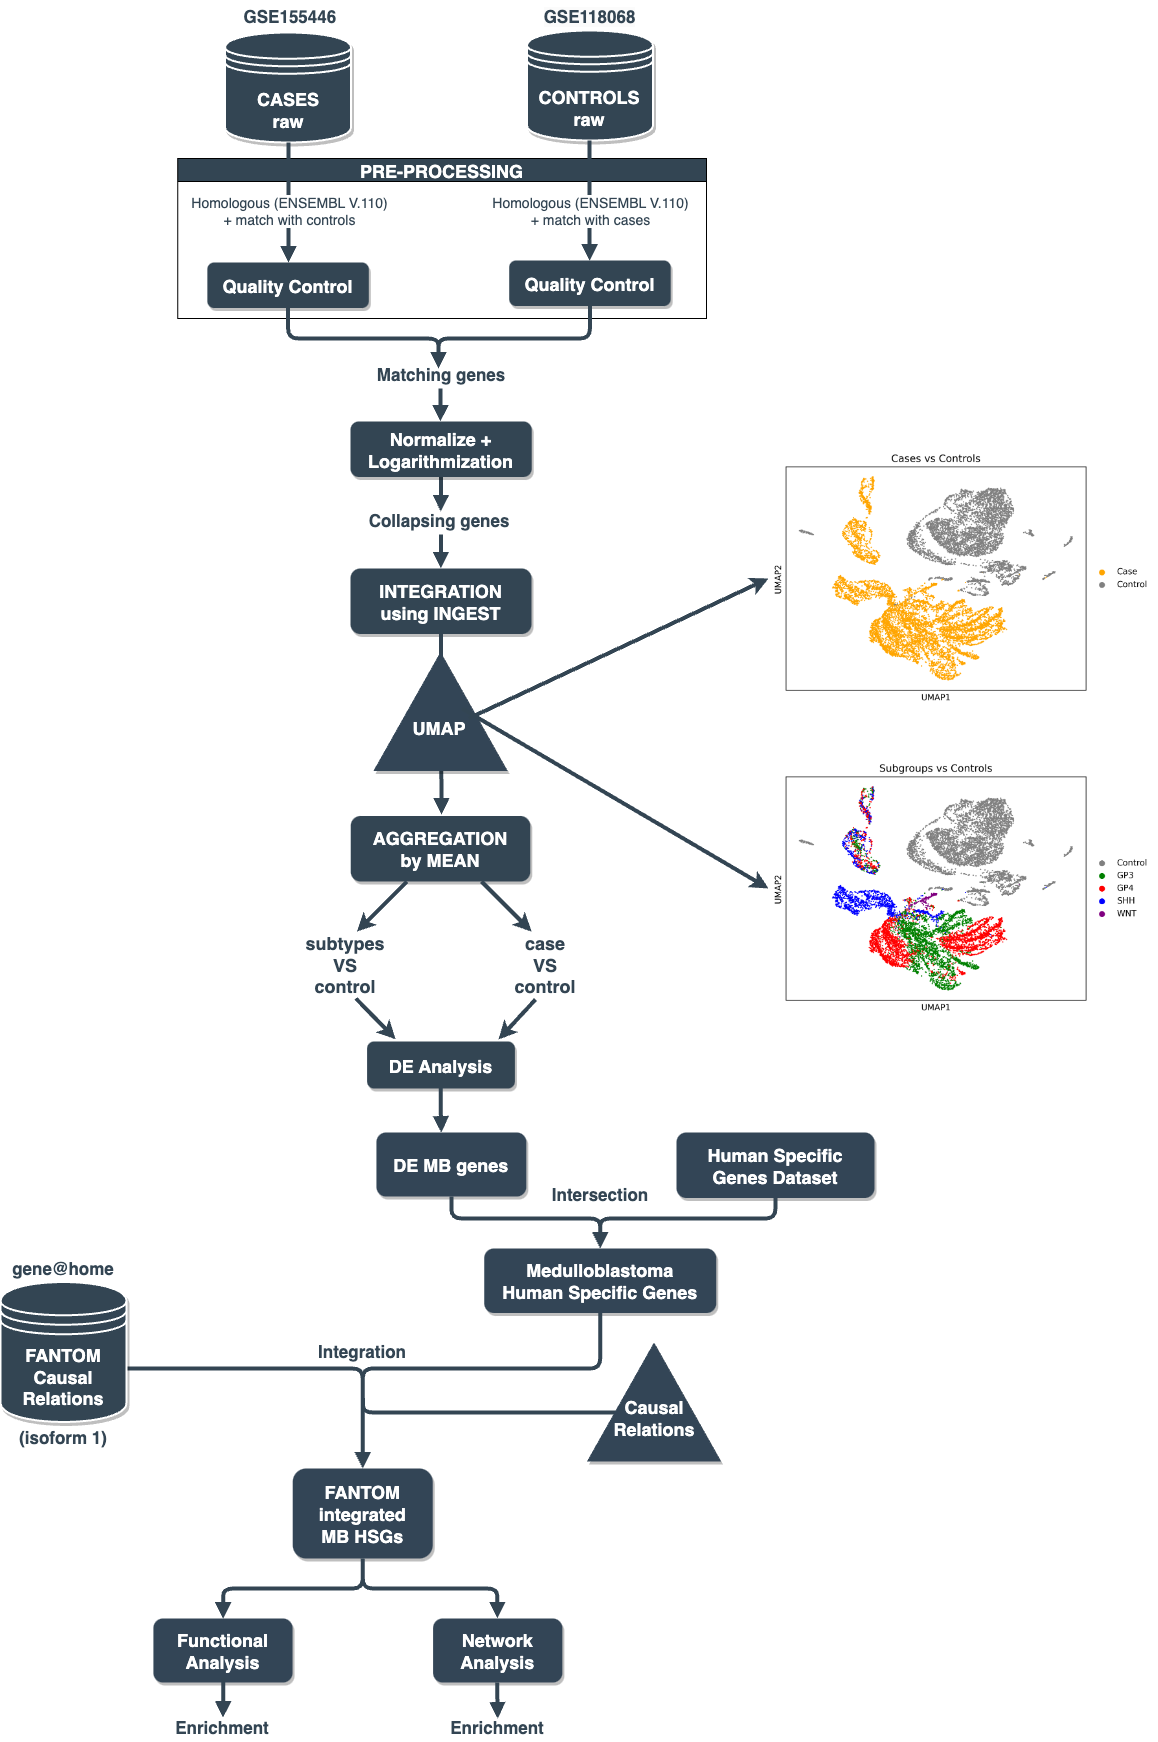
\includegraphics[width=0.72\textwidth]{project-report/figures/pipeline.png}
    \caption{General workflow depicting the main steps of the project.}
    \label{fig:pipeline}    
\end{figure}

\newpage
\section{Results}\label{sec:results}
\subsection{Homologous Gene Filtering}\label{sec:homologous_results}
In the initial phase of homologous gene identification, we sought to establish orthologous relationships between human and murine genes. Following the mapping using Ensembl (v.110) \cite{biomart_ensembl110}, the results revealed a total of $15180$ homologous genes in the human dataset and $16866$ genes in the murine dataset.
Subsequently, to ensure consistency and compatibility between the two datasets, we performed a refined filtering step to identify and retain only the homologous genes present in both datasets. After applying this filtering criterion, $14524$ homologous genes were identified as shared within the two matrices. 


\subsection{Quality Control}\label{sec:quality_results}
\subsubsection*{GSE155446}
After the QC procedures, the GSE155446 dataset retained $38598$ cells and $14219$ genes. 
Following this process, an insightful observation emerged. Notably, the cells that did not pass the QC set by applying thresholds were consistent with those identified when initially considering the entire dataset. 

\subsubsection*{GSE118068}
As with the GSE155446 dataset, the threshold values for these filters were determined by analyzing the distribution of occurrences and the percentage of mitochondrial genes for each cell. 
Post-QC, the GSE118068 dataset retained $26914$ cells and $14484$ genes. 
As proof of concept, also in this case a parallel observation was made: the cells that did not meet the QC criteria established through threshold analysis were found to be the same as those identified when the dataset was considered in its entirety.

\subsection{Data Filtering for Common Genes}\label{sec:fltering_common_results}
Due to QC measures, a subset of genes in both datasets did not meet the defined criteria and were subsequently filtered out.
To maintain consistency and comparability post-QC, we performed a secondary data filtering step specifically targeting common genes between the human and murine datasets. \\
As a result of refiltering step, $13477$ genes were identified as common homologous genes shared within the two matrices. However, some genes from the murine dataset were found to map for more than one gene in the human cohort. For this reason, a genes collapsing strategy was employed after the normalization process. 

\subsection{Data Normalization}\label{sec:normalization_results}
A data normalization step was applied to both the two datasets in order to mitigate technical biases and promoting data comparability. \\
The target sum for each cell was set to $1e4$, ensuring a comparable representation across individual cells. Subsequently, a logarithmic transformation was applied using \textit{log1p} function. \\

\subsection{Genes Collapsing}\label{sec:genes_collapsing_results}
In response to instances where multiple murine genes mapped to the same human gene, we implemented a gene collapse strategy. This involved aggregating expression values of these genes by calculating their mean expression. \\
As a result, we obtained two matrices, each with a consistent and unified set of genes. In total $13477$ unique genes were retrieved for both the two datasets. In \textbf{Figure \ref{fig:GSE_normalized}} the UMAP of the pre-processed dataset is shown.

\begin{figure}[H]
    \begin{minipage}{0.48\textwidth}
        \centering
        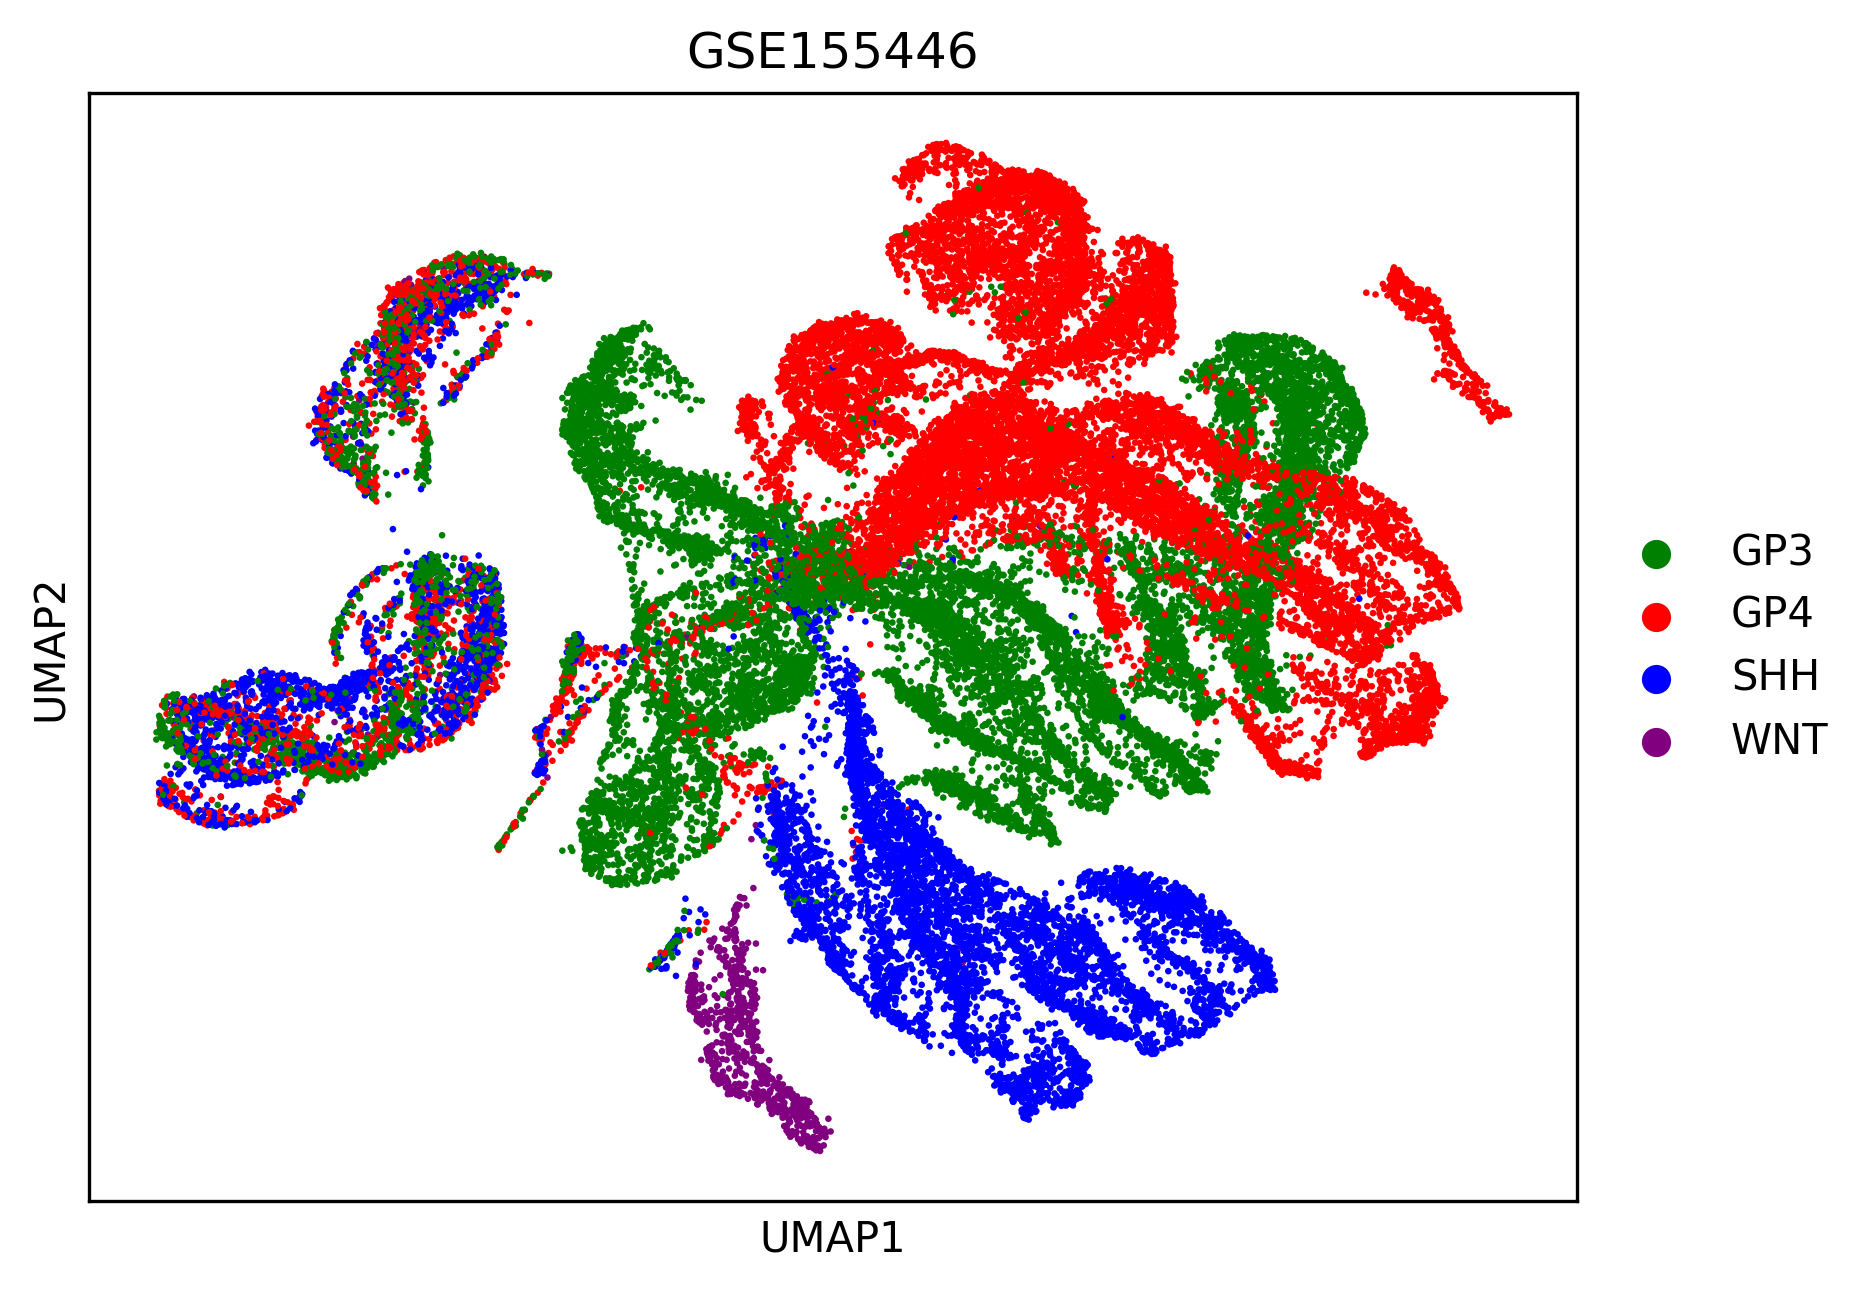
\includegraphics[width=\textwidth]{project-report/figures/umap/GSE155446_umap_plot_def.png}
    \end{minipage}\hfill
    \begin{minipage}{0.48\textwidth}
        \centering
        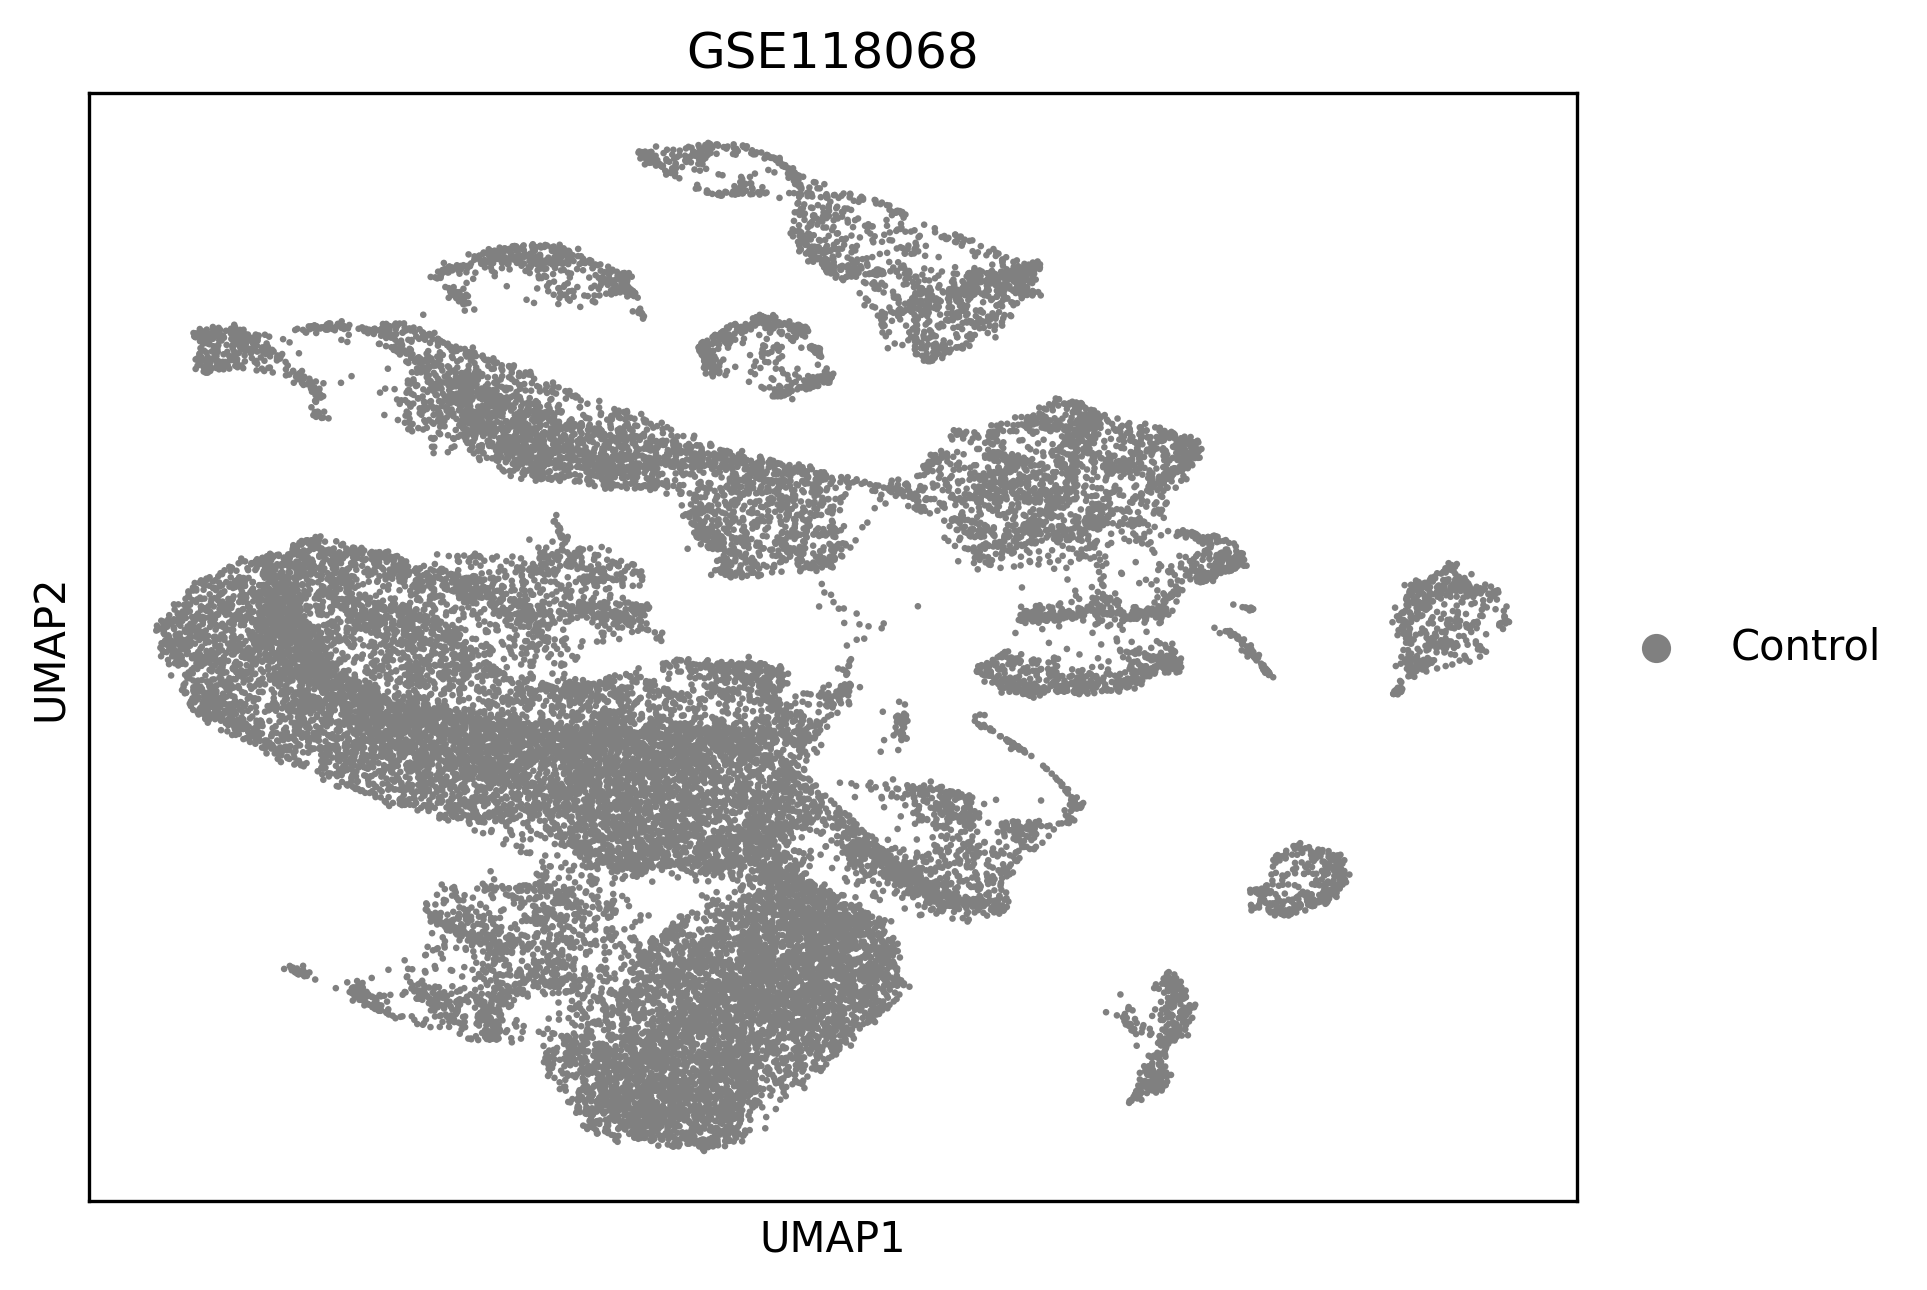
\includegraphics[width=\textwidth]{project-report/figures/umap/GSE118068_umap_plot_def.png}
    \end{minipage}
    \caption{UMAP plots of pre-processed data from two distinct datasets: GSE155446 (MB - GP3, GP4, WNT, SHH) and GSE118068 (controls). These visualizations depict dimensional reduction through UMAP after pre-processing of gene expression data.}
    \label{fig:GSE_normalized}
\end{figure}

\subsection{Datasets Integration}\label{sec:integration_results}
The integrated dataset is composed of $65506$ cells and $13477$ genes. In \textbf{Figure \ref{fig:GSE_integrated}} the UMAP of the integrated dataset is shown. 

\begin{figure}[H]
    \begin{minipage}{0.48\textwidth}
        \centering
        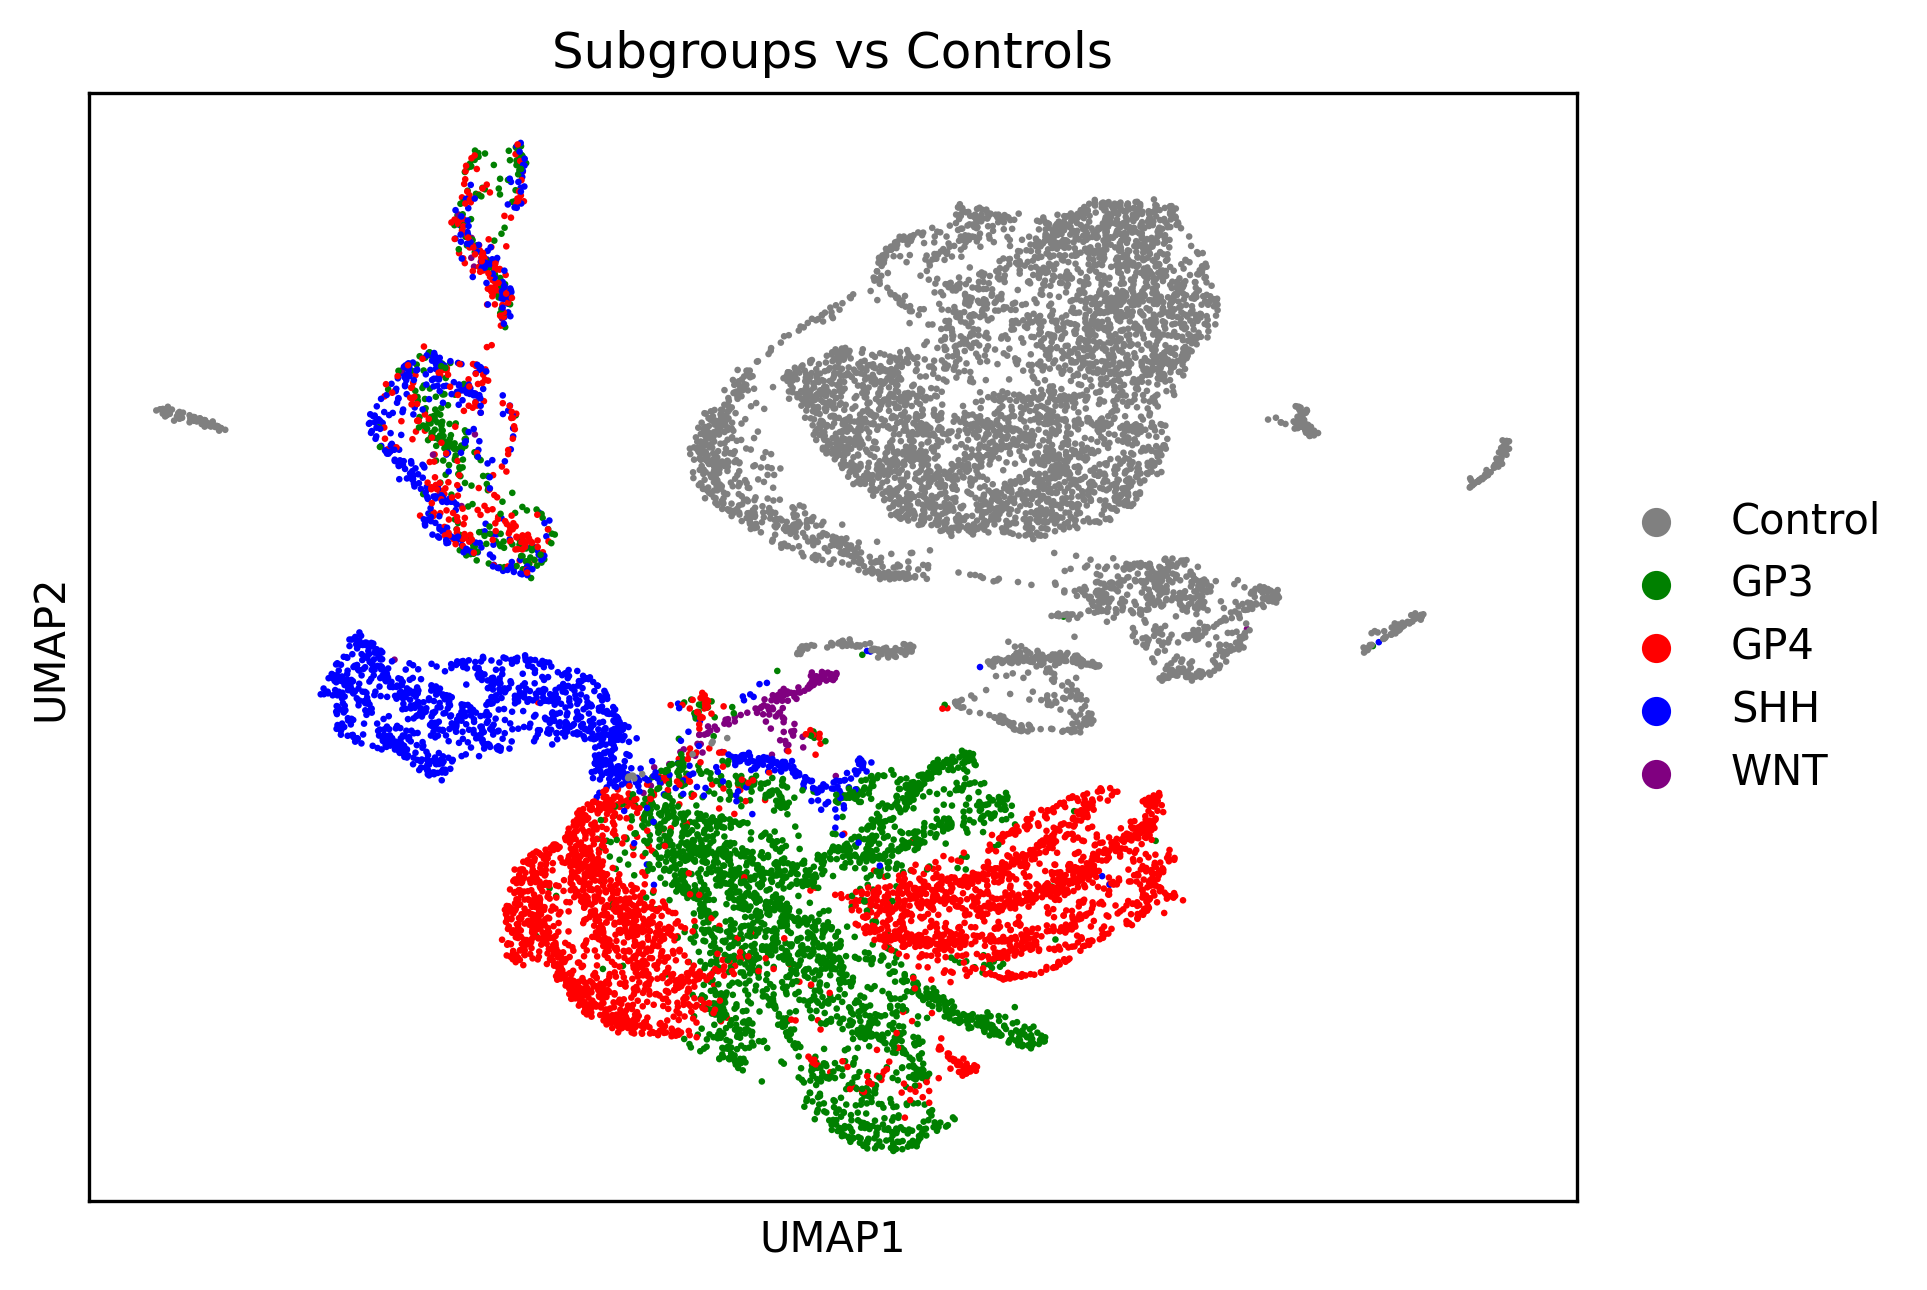
\includegraphics[width=\textwidth]{project-report/figures/umap/GSE_integrated_umap_subtypes_controls.png}
    \end{minipage}\hfill
    \begin{minipage}{0.48\textwidth}
        \centering
        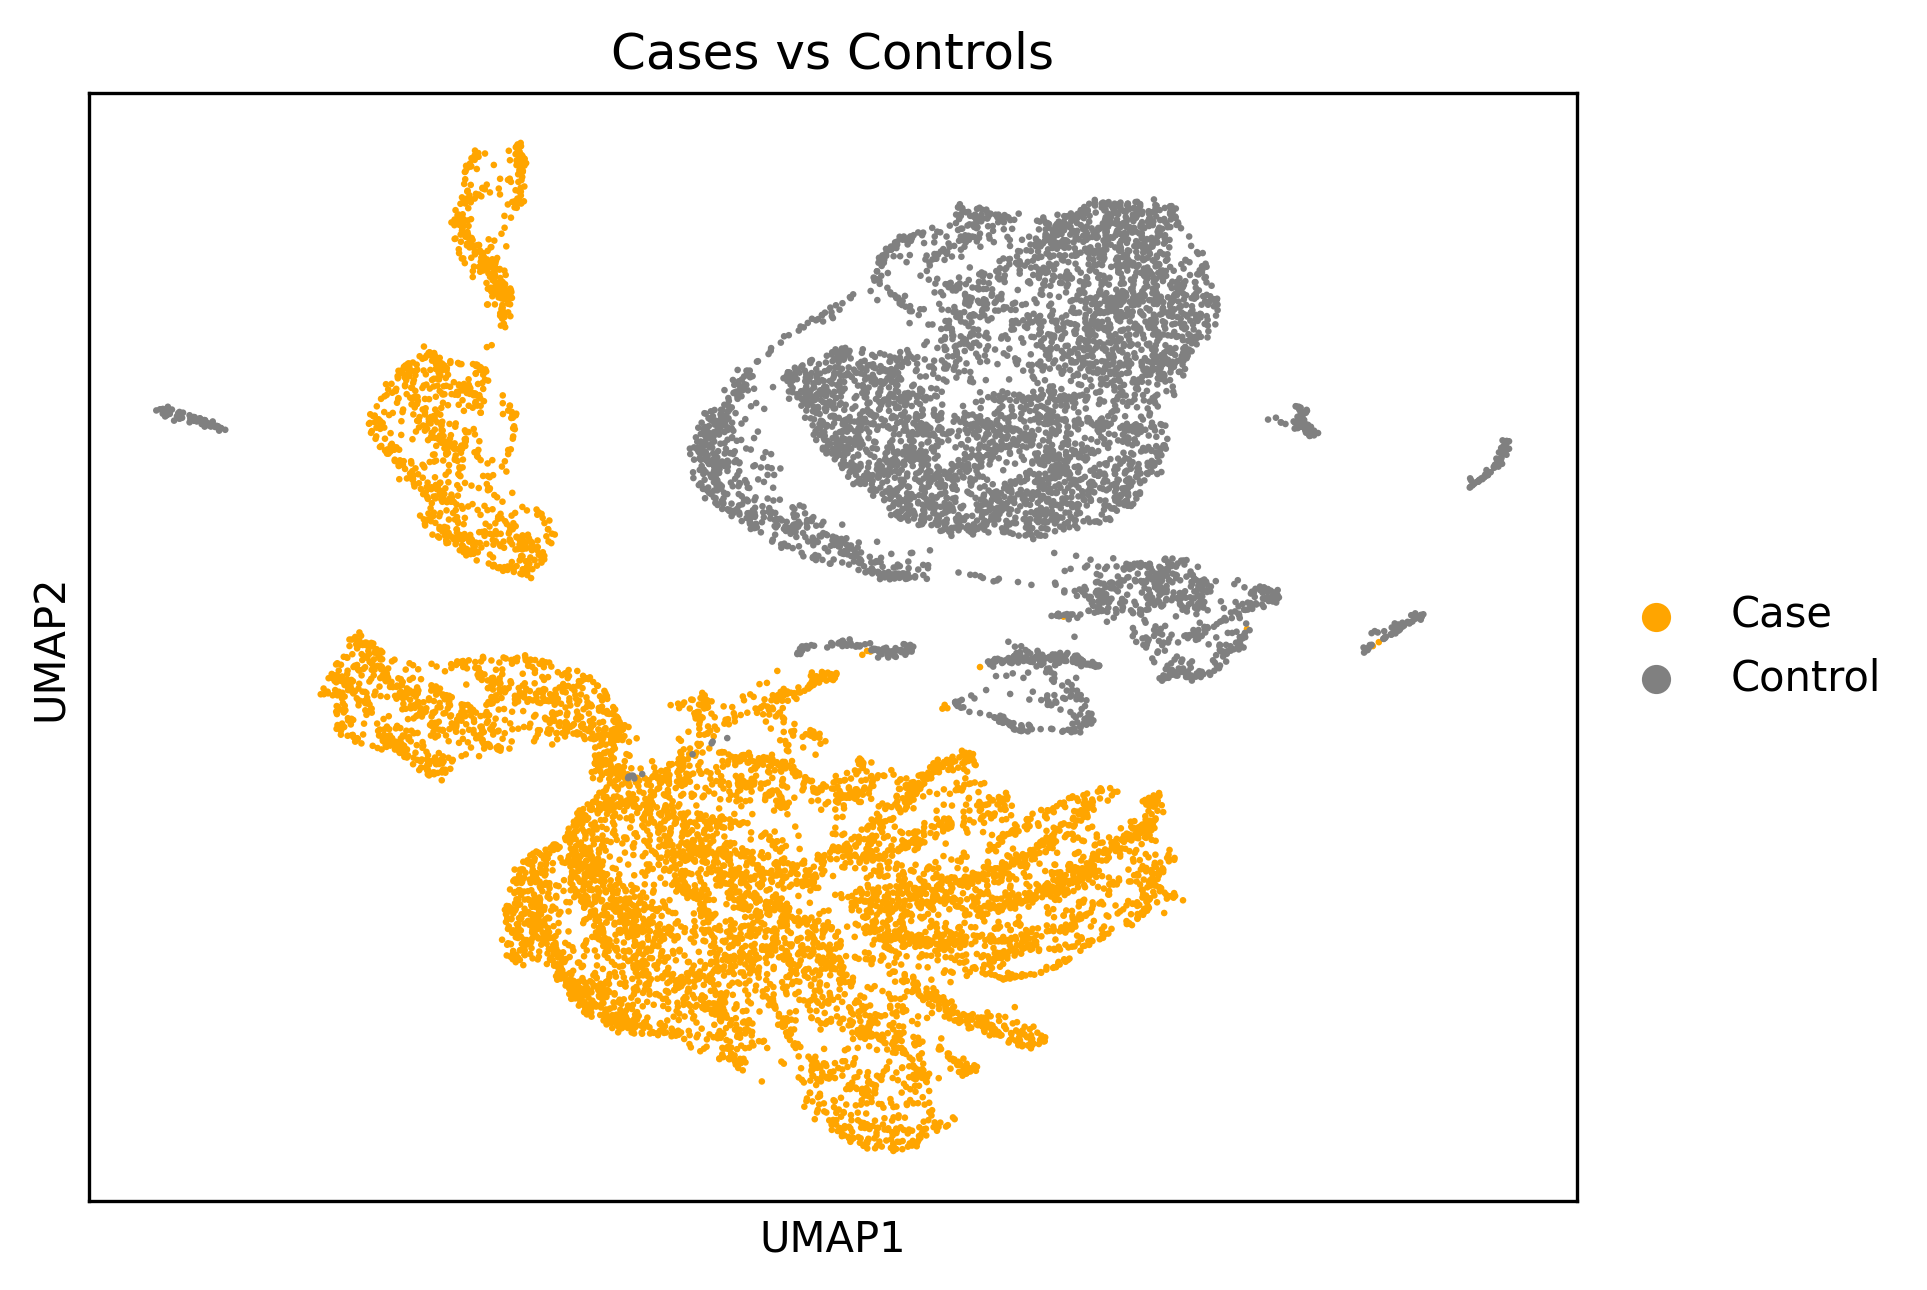
\includegraphics[width=\textwidth]{project-report/figures/umap/GSE_integrated_umap_cases_controls.png}
    \end{minipage}
    \caption{The UMAP plots of the integrated dataset were generated by sampling $80\%$ of the cells from the entire matrix, while maintaining the proportions of composition.}
    \label{fig:GSE_integrated}
\end{figure}


\subsection{DE Analysis}\label{sec:DE_results}
The DE Analysis outputted adjusted p-values and fold changes for all $13477$ genes. Those were used to build the volcano plots (\textbf{Figure \ref{fig:panel_volcano}}): firstly by considering all genes and secondly by plotting only the human specific ones. The filtering procedure applied to cases and subgroups outputted what we ultimately refer to as hit genes, used in both Network and Functional analysis and highlighted in the volcano plots (\textbf{Figure \ref{fig:panel_volcano}}, second column).
The difference between the quantity of up and down-regulated genes is distinguishable when comparing cases against the four subtypes.

\begin{figure}[h!]
    \centering
    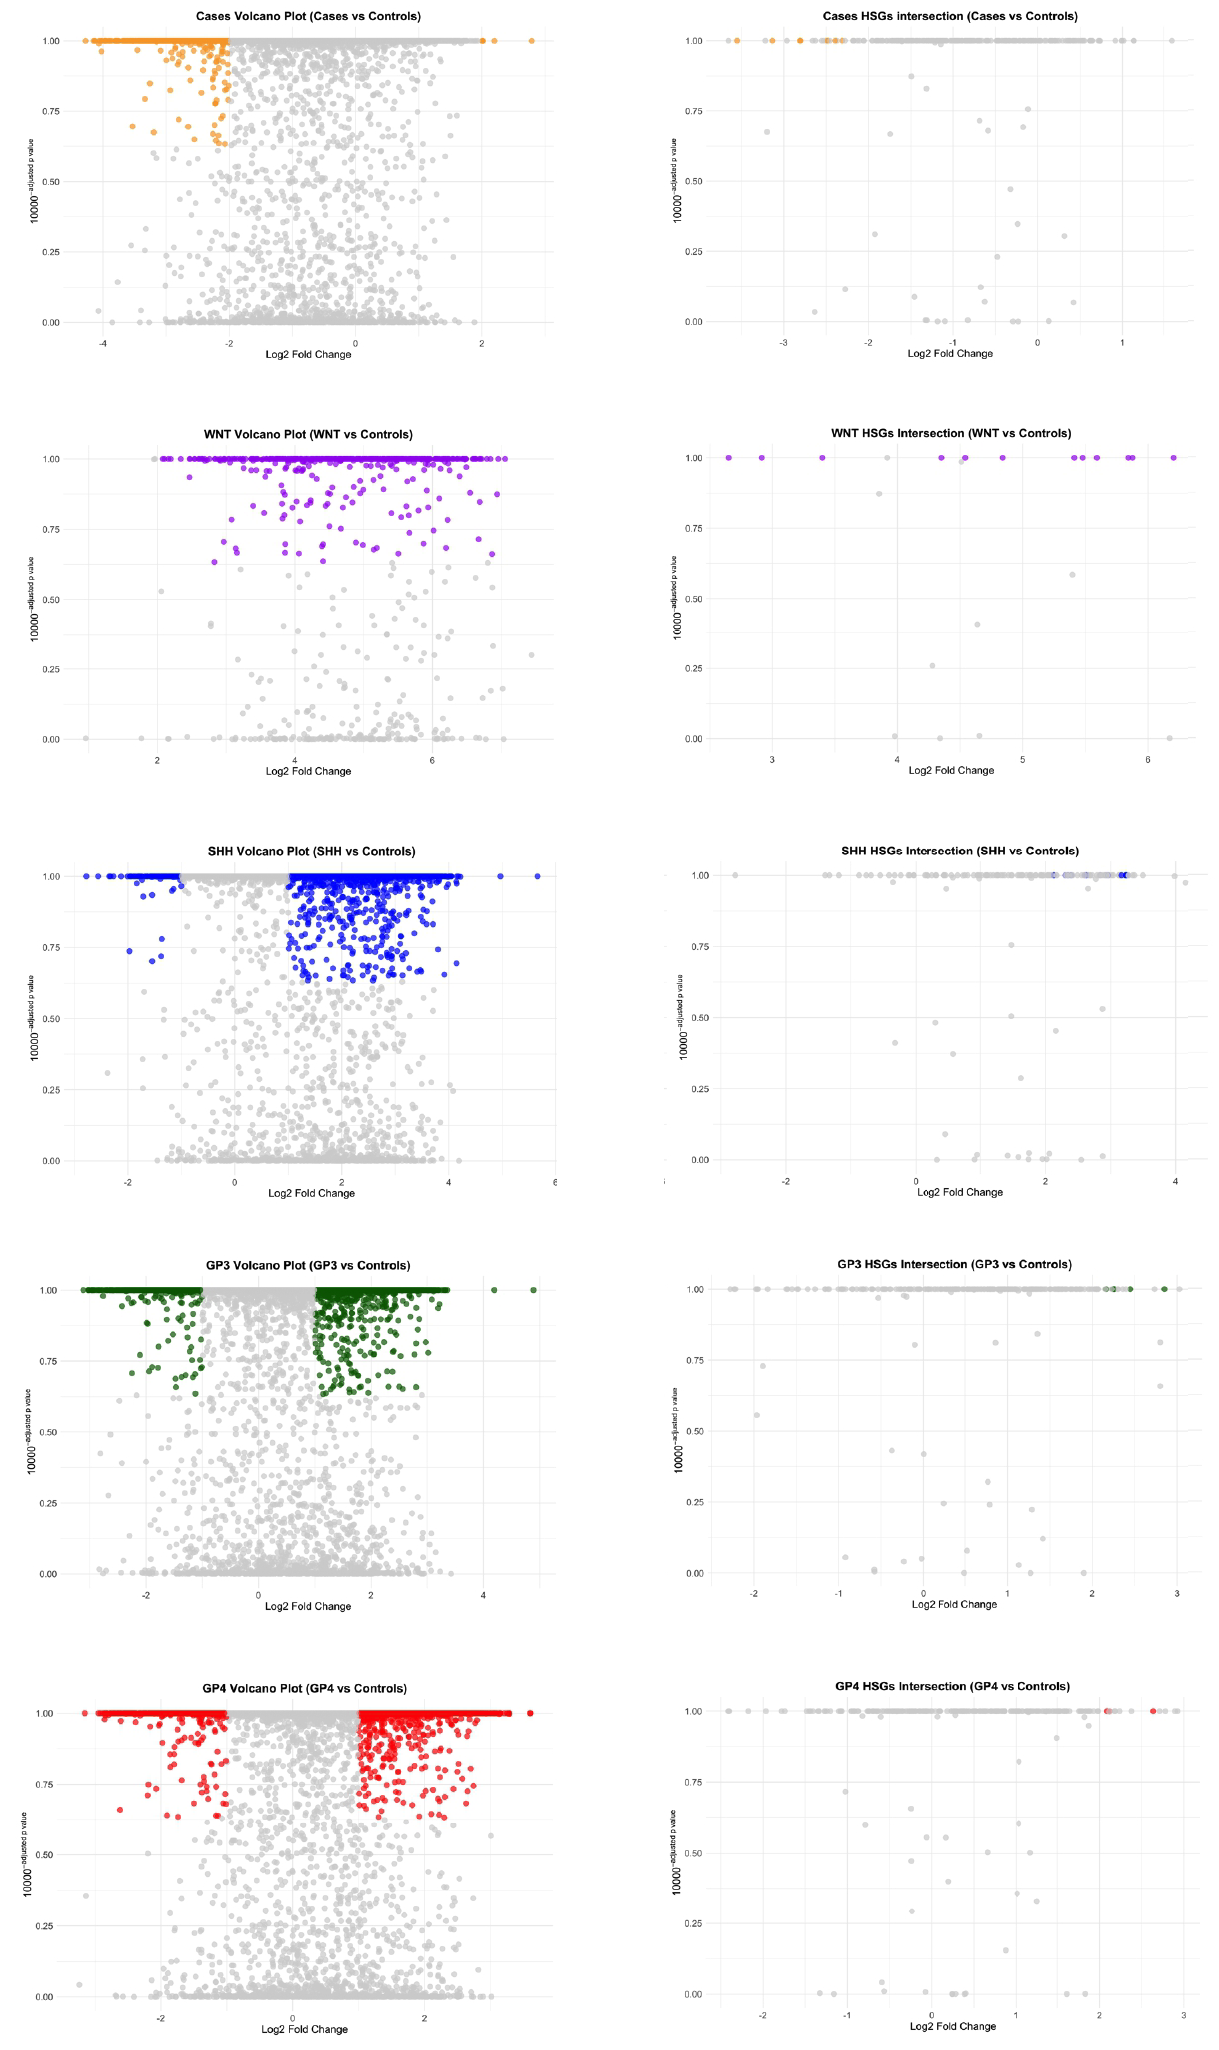
\includegraphics[width=0.75\textwidth]{project-report/figures/volcano_panel2.png}
    \caption{Panel displaying the 5 different volcano plots for the DE analysis. In order: Cases, WNT, SHH, Gp3, Gp4.}
    \label{fig:panel_volcano}    
\end{figure}

\subsection{Network Analysis}\label{sec:network_results}
By expanding with FANTOM \cite{fantom5} causal relations our hit genes, we ended up building 4 small networks in order to gain further knowledge regarding whether our human specific hit genes were causally related to one another with bridge-like causal relations. The size of the nodes is directly proportional to their betweenness centrality measure and logically the hit genes are represented as community hubs surrounded by the cloud of FANTOM \cite{fantom5} genes and sometimes connected to one another either via intermediate genes or, less often, directly.\\
WNT and SHH subgroups (\textbf{Figure \ref{fig:network_panel}c,d}) have more complex networks due to them having a higher number of hit genes passing through the filtering and FANTOM \cite{fantom5} integration. Out of the three Gp3-HSGs (\textbf{Figure \ref{fig:network_panel}b}), two had the bridge gene \textit{KCNAB2} connecting them. Note that the Gp4 MB subgroup network is missing due to the absence of causal relations connecting differentially expressed HSG.


\begin{figure}[h!]
    \centering
    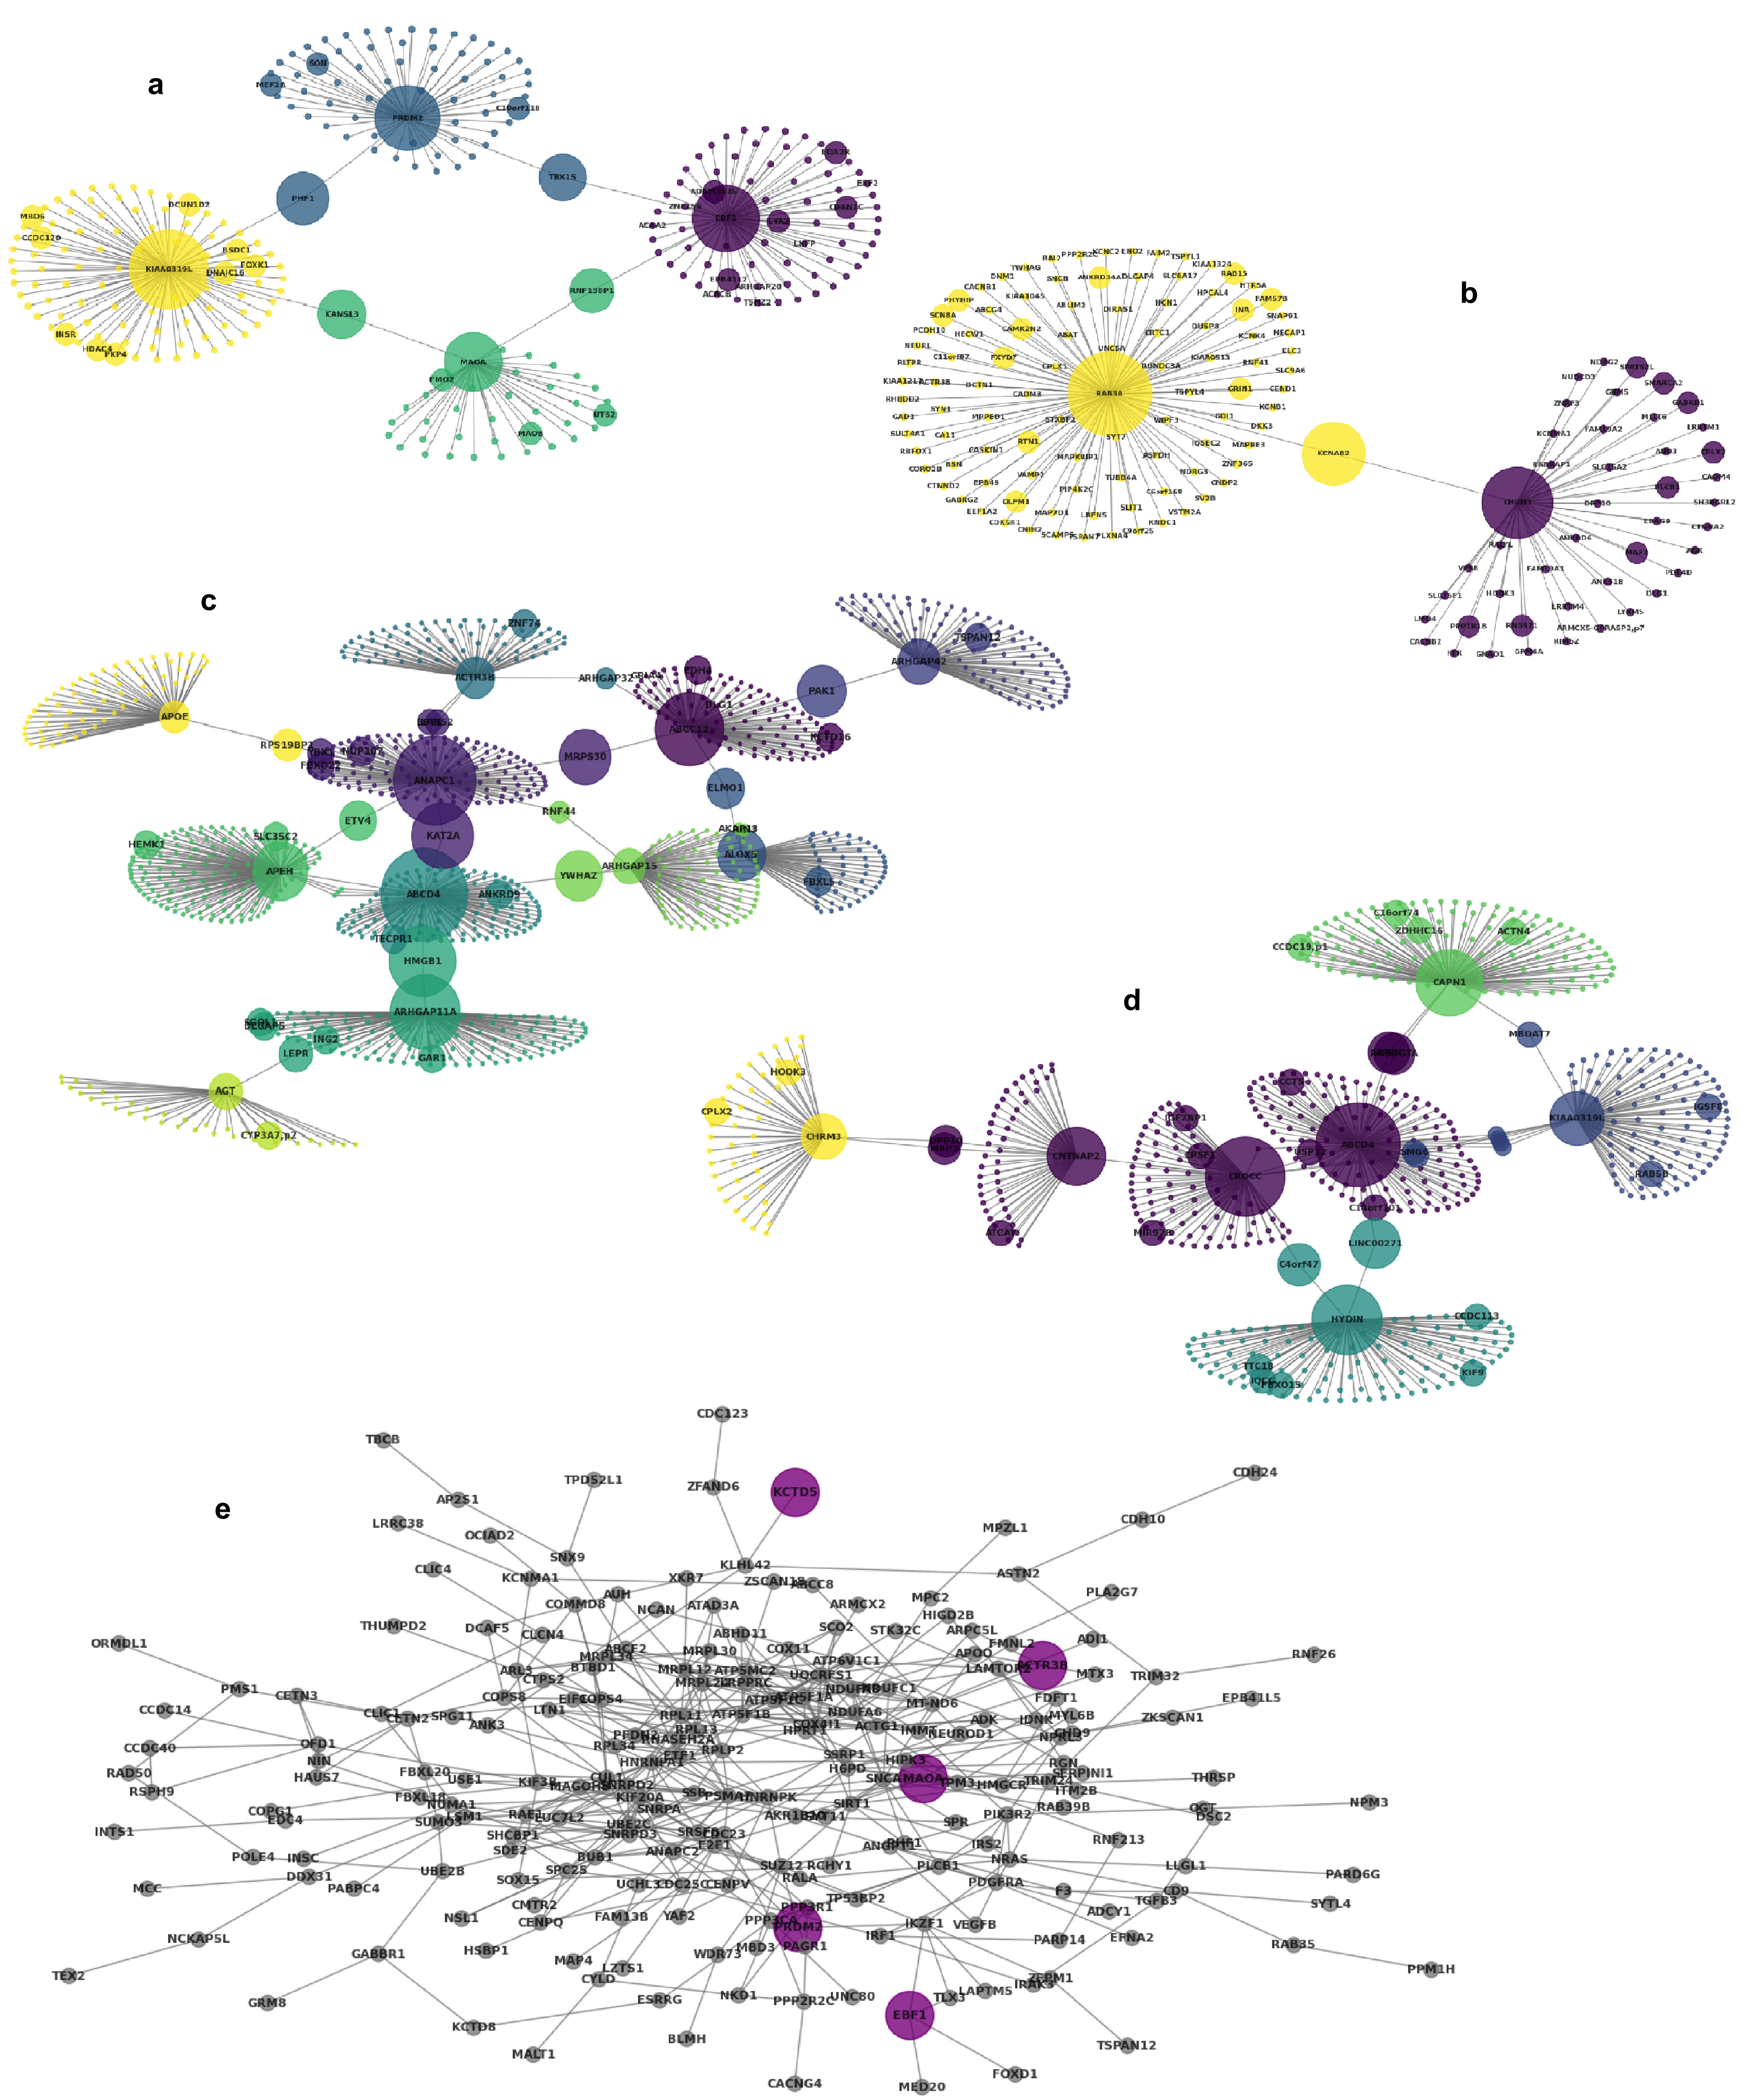
\includegraphics[width=0.96\textwidth]{project-report/figures/network_panel2.png}
    \caption{Panel depicting the 5 networks of our analysis. \textbf{a}. Network of the cases group intersected with HSGs; \textbf{b}. Newtork of the Gp3 subtype intersected with HSGs; \textbf{c}. Newtork of the WNT subtype intersected with HSGs; \textbf{d}. Newtork of the SHH subtype intersected with HSGs; \textbf{e}. Newtork representing all the cases, where the HSGs were highlighted. (High quality versions of the images are available in the Supplementary Material.)}
    \label{fig:network_panel}    
\end{figure}

Despite the fact that some HSGs did not have edges connecting them or other intermediate genes, they were kept for functional analysis and treated equally together with their FANTOM \cite{fantom5} causal relations.\\
Using the complete list of case-DE genes we built a network (\textbf{Figure \ref{fig:network_panel}e}) by retrieving edges with STRING \cite{szklarczyk2019string} and highlighting the presence of 5 HSGs out of the total of 8 previously found.

\subsection{Functional Analysis}\label{sec:functional_results}
After gaining an overview on STRING \cite{szklarczyk2019string} about which specific terms to look for in other databases, we looked for diseases associated to our genes on Enrichr \cite{kuleshov2016enrichr}: all five gene sets showed a prevalence of neuro-related diseases such as epilepsy, mental retardation, intellectual disability and seizures.
We then investigated the localization of the gene sets finding that all of them were significantly expressed in the brain and in the cerebellum. These results yielded highly significant with p-values of: 10\textsuperscript{-10}, 10\textsuperscript{-18}, 10\textsuperscript{-8}, 0.009, and 10\textsuperscript{-9} respectively for SHH, WNT, Gp3, Gp4 and cases.\\
Lastly, through the pathway enrichment analysis we observed a trend characterizing our genes. The cases and Gp3 sets showed involvement in pathways related to the neuronal system and brain functions. SHH, WNT, and Gp4 gene sets were found to participate in cell cycle pathways known to be, if altered, one of the major causes of tumors.\\
These analyses led us to acknowledge the importance of the involvement of the FANTOM \cite{fantom5} expanded DEGs in brain functions and localization.\\
Tables retrieved from Enrichr \cite{kuleshov2016enrichr} and from Reactome Pathway Database \cite{gillespie2022reactome} can be found in the Supplementary Material.

\begin{figure}[h!]
    \centering
    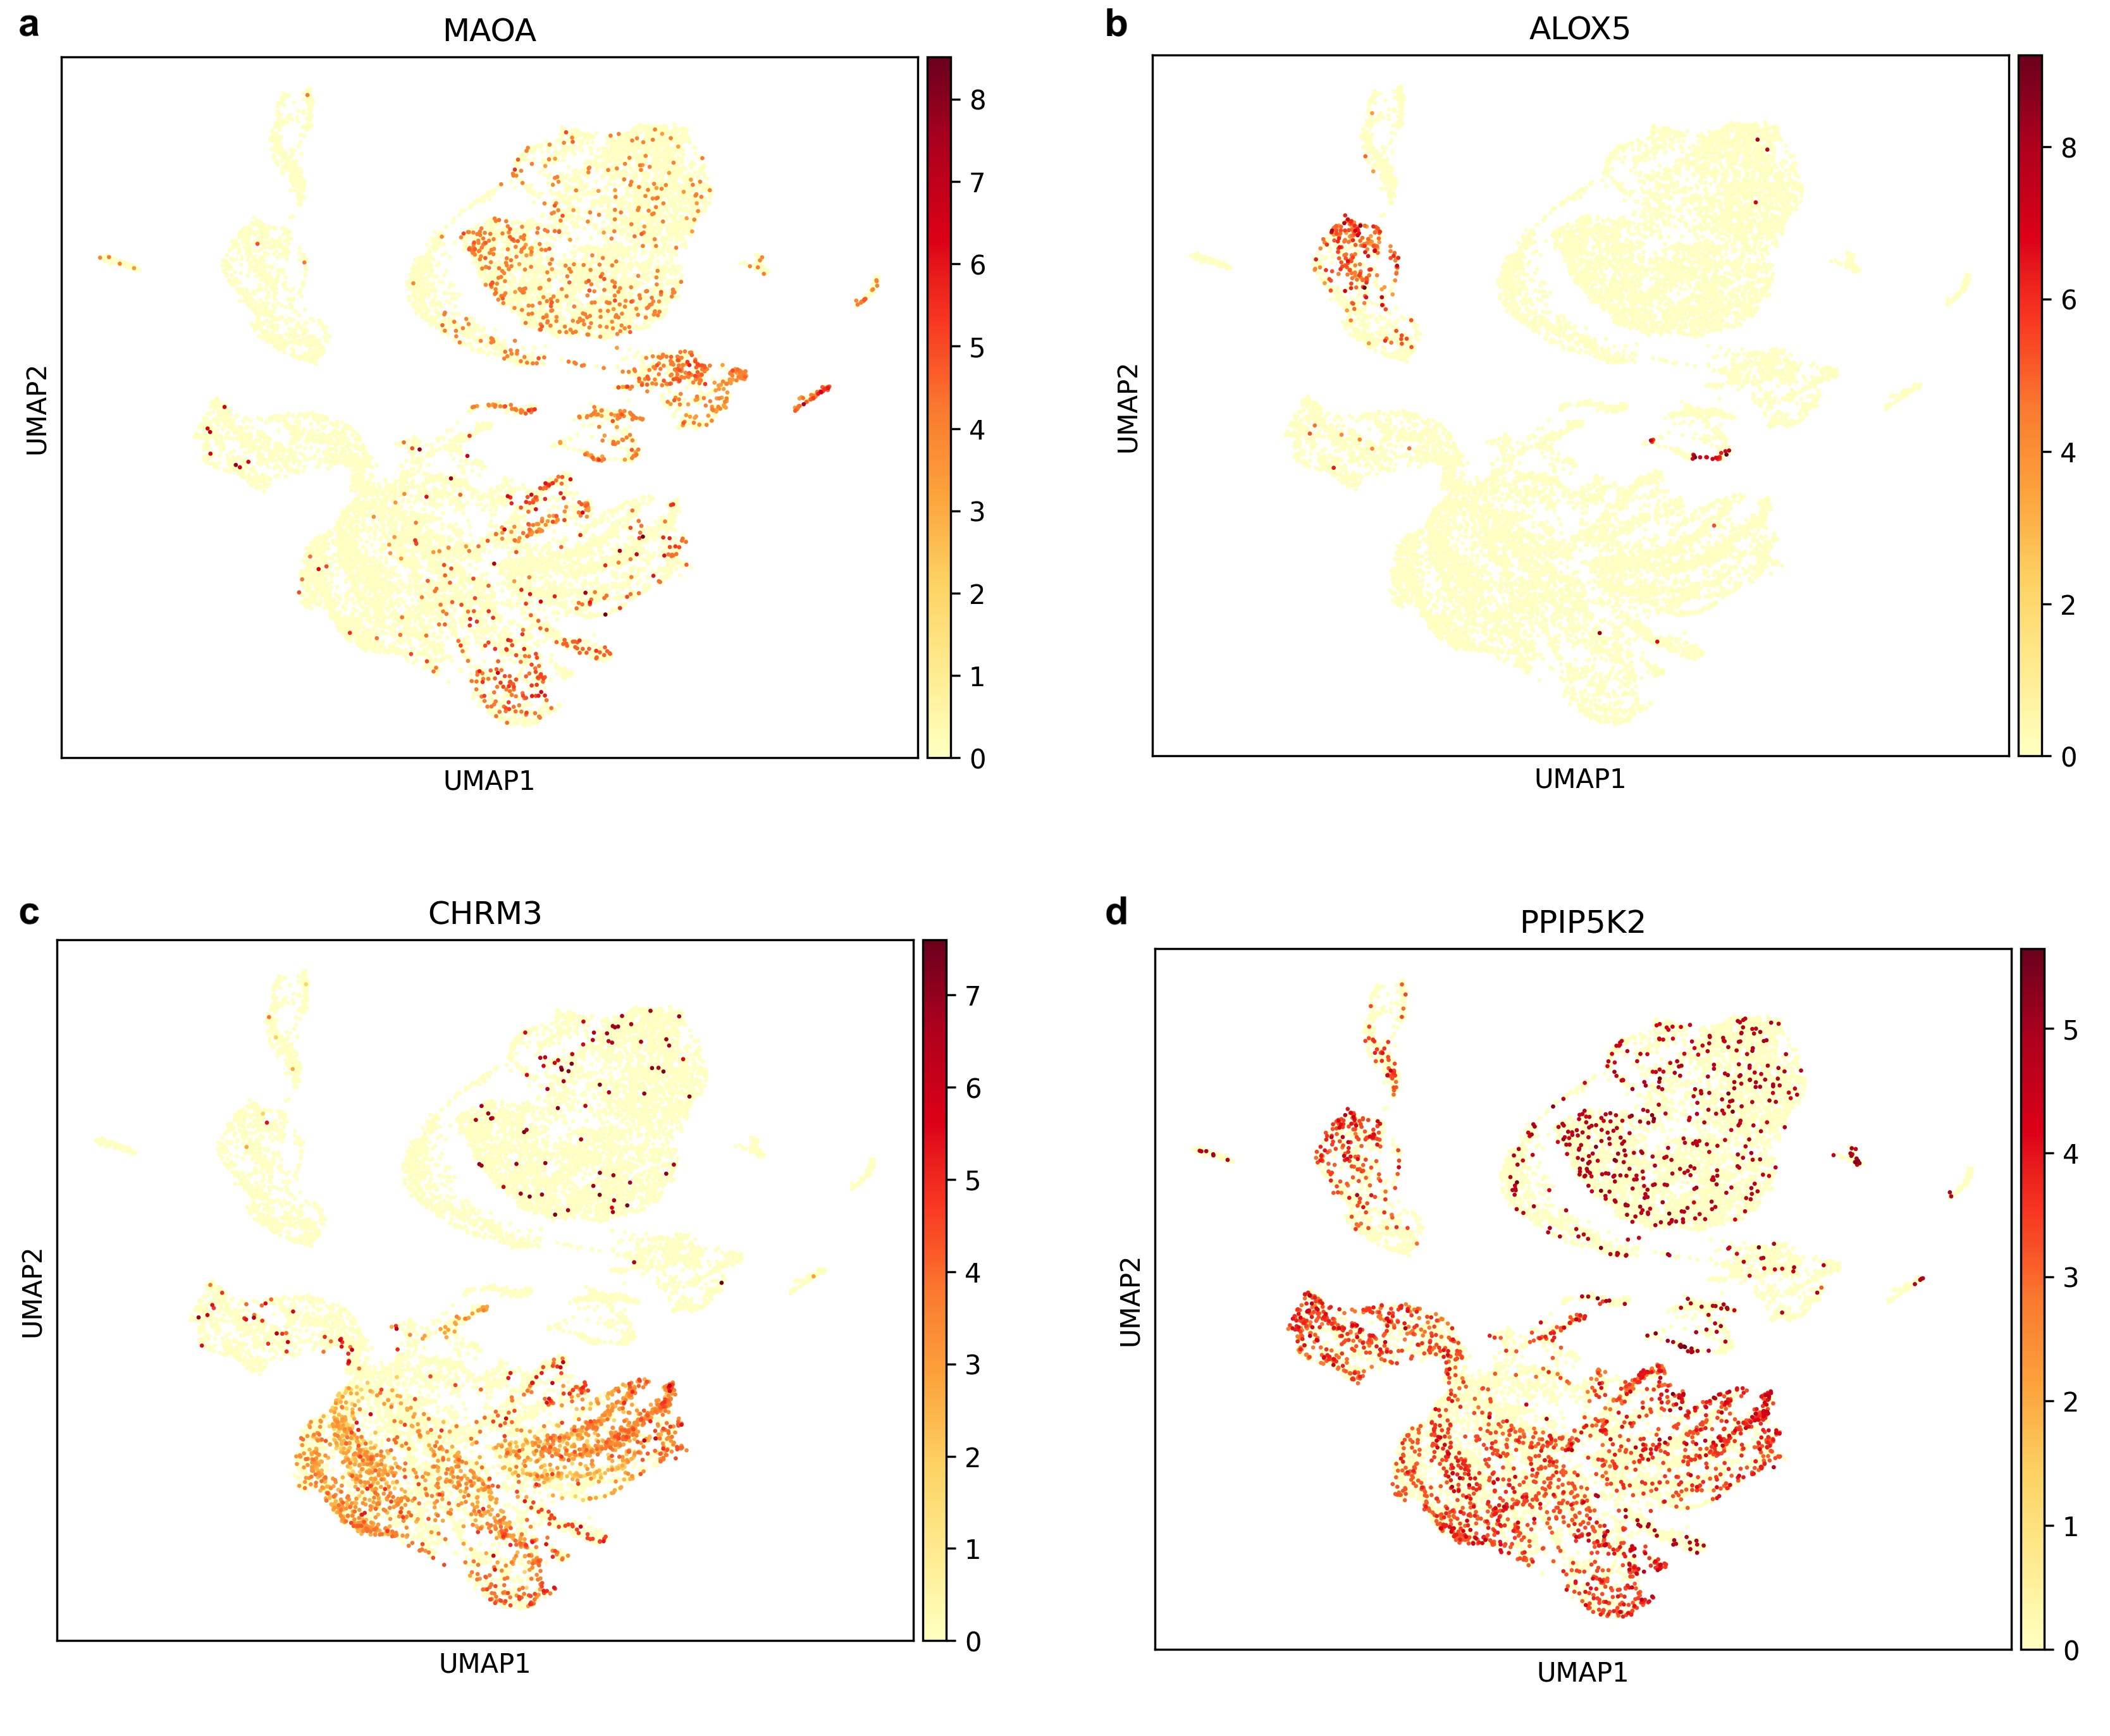
\includegraphics[width=1\textwidth]{project-report/figures/umap/UMAP_panel.png}
    \caption{Panel displaying the UMAP-heatmaps of 4 hit genes: \textbf{a}: MAOA (for cases), \textbf{b}: ALOX5 (for WNT), \textbf{c}: CHRM3 (for Gp3 and SHH) and \textbf{d}: PPIP5K2 (for Gp4)}
    \label{fig:umap_panel}    
\end{figure}

\section{Discussion}\label{sec:discussion}
Starting from a MB cases matrix and a control one, we performed a pre-processing pipeline and a DE Analysis. We obtained a set of HSGs that with a very high confidence were differentially expressed between MB cases and controls or among the four MB subgroups versus controls. Indeed, the Benjamini-corrected p-values turned out to be very low: the lowest ones were in the order of $-300$ or less and they were collapsed to the zero value. Although they might seem extremely low, it is reasonable to obtain such p-values since the distribution comparison that is performed during the DE analysis is applied to around $30.000$ samples (\textbf{Table \ref{tbl:sample_sizes}}).\\

\begin{table}[h!]
  \label{tbl:sample_sizes}
  \centering
    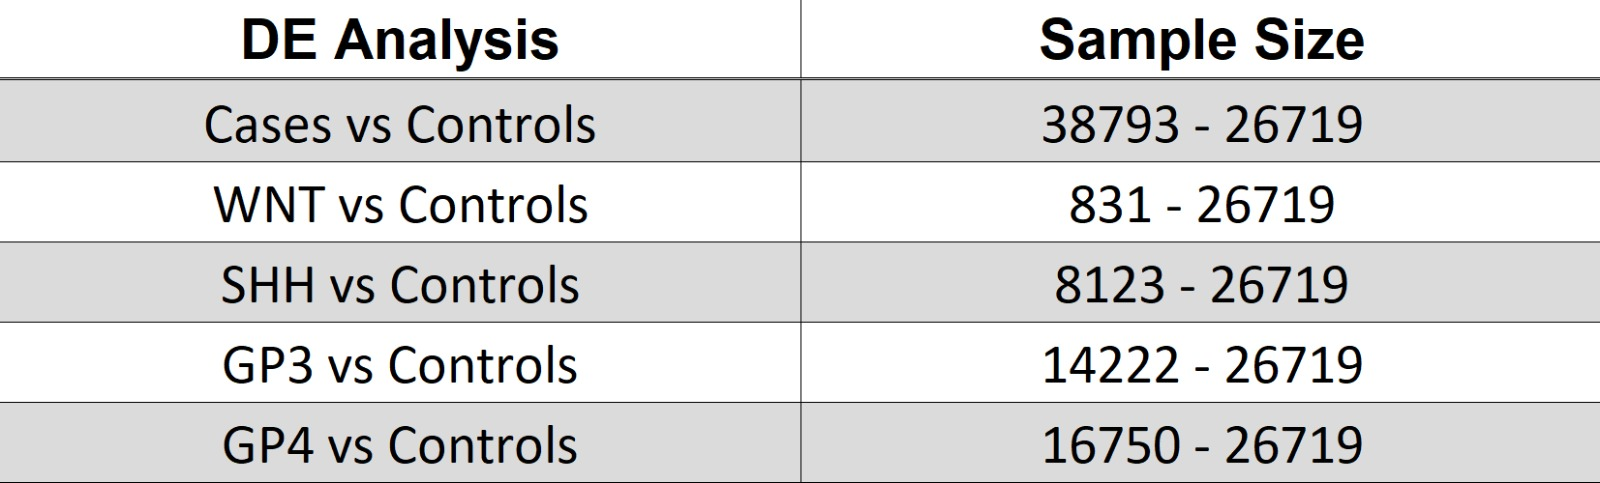
\includegraphics[width=0.6\textwidth]{project-report/figures/sample_sizes.jpeg}
    \caption{Number of samples used for each DE Analysis: respectively cases and subtypes against controls.}  
    \label{tbl:sample_sizes}
\end{table}

Regarding the distribution of the p-values visible from the volcano plots (\textbf{Figure \ref{fig:panel_volcano}}), the crowding of points in the values 0 and 1 corresponds to robustness in our statistical test. Having many samples to compare one against the other, the Wilcoxon-Mann-Whitney test manages to separate with high degree of certainty the genes that are differentially expressed and those that are not, with fewer hits in the uncertain area. \\
We noticed a widespread down-regulation of genes in MB cases. There could be two possible reasons for this: first, it could be that these genes are naturally more active during pre-natal development rather than after birth like in our samples; second, there might be a technical problem affecting the data.
On the other hand, the four subgroups show a prevalence of up-regulated genes suggesting that there could be a set of them expressed during the post-natal phase (\ref{sec:GSE118068} GSE118068) specific to each MB subgroup.\\
From the UMAP plots (\textbf{Figure \ref{fig:GSE_integrated}}), we can observe that cases and controls are well separated, with few overlaps. The distinction between the four MB subtypes is noticeable, with some intersection regions including all of them. These two observations constitute a solid basis to build our results on.\\
Based on the outcomes of the DE Analyses and on the topology of the networks (\textbf{Figure \ref{fig:network_panel}}), some HSGs and intermediate genes have been selected for subsequent in-depth investigations. \\

\subsection{Cases DEGs}\label{sec:cases_DE}
\textit{PRDM2}, which was found to exhibit low expression in MB cases, is a histone 3 lysine 9 methyltransferase. The low expression level of this gene is in accordance with its role of tumor suppressor gene. It is usually low expressed in MB Group 3 compared to other subgroups \cite{stripay2019medu}; unexpectedly the \textit{PRDM2} gene is up-regulated in GP3 subgroup according to our data.\\
The \textit{TBX15} gene, acting as a non-HSG bridge in the cases network and causally linked to \textit{PRDM2} has also been related to a variety of tumors \cite{yan2023overexpression} when up-regulated, in agreement to our cases sample.\\
\textit{MAOA} was also found to have a significantly low expression level in MB patients. \textit{c-Myc}, a well known oncogene which is capable of promoting MB development, induces the expression of the \textit{R1} gene that is able in turn to potentiate the effect of \textit{c-Myc} on MB by increasing its stability. At the same time, the \textit{R1} gene inhibits \textit{MAOA} mRNA levels \cite{ou2006monoamine}. As a result, we described a pathway in which the \textit{R1} gene is responsible both for enhancing cell proliferation and MB development through \textit{c-Myc} stabilization and for inhibiting \textit{MAOA} expression levels. This is coherent with our findings since the under-expression of the \textit{MAOA} gene, also visible in our UMAP-heatmap (\textbf{Figure \ref{fig:umap_panel}a}), has been demonstrated to be correlated with a high expression of the MB-related \textit{c-Myc} oncogene.\\

\subsection{WNT DEGs}\label{sec:WNT_DE}
The \textit{ALOX5} gene, which resulted to be up-regulated in the MB WNT group, is responsible for Leukotrienes syntesis together with 5-lipoxygenase-activated protein (\textit{FLAP}). Leukotrienes are inflammatory mediators that, besides having a wide range of biological functions including astrocyte proliferation, are also highly synthesized in MB cells. This happens through the production by Leukotrienes of Nestin, an intermediate filament protein required for MB progression \cite{du2019leukotriene}. Intuitively, blocking \textit{ALOX5} expression could impair Nestin production and hence MB progression; it was indeed discovered that mutating the \textit{ALOX5} gene, a markedly prolonged tumor latency was observed \cite{du2019leukotriene}. Hence, the discovery of \textit{ALOX5} high expression level in the MB WNT subgroup (\textbf{Figure \ref{fig:umap_panel}b}) confirms the role of this gene in MB progression through Leukotrienes production and suggests us to consider this gene as a candidate biomarker for the WNT group. To elucidate this hypothesis, further studies are needed. Moreover, the \textit{ALOX5} gene could be experimented as a drug target for impairing MB advancement. Causally linked to \textit{ALOX5}, \textit{ELMO1}, a non-HS down-regulated gene, is also reported to be a MB-related gene and potential biomarker \cite{liu2020identification}. \\
Following, the non-human specific \textit{PAK1} gene, which resulted from the FANTOM \cite{fantom5} integration, was found to be up-regulated in the MB WNT subgroup and it plays an important role in MB cell migration \cite{yuan2010erk}. Phosphorylation of Thr212 and Thr423 on \textit{PAK1} by \textit{ERK} in response to \textit{PDGF} correlates with the functional activities of MB cells. The \textit{PDGFR}-\textit{ERK} signaling is relevant for MB growth and metastasis and it was also proven that their regulation towards the \textit{PAK1}-\textit{RAC1} signaling is linked to \textit{PDGF}-mediated MB cell migration. Additionally, the \textit{PDGFR} gene is also present in our cases DEGs, whose abnormal signaling can lead to disruptions in neuronal migration and normal cerebellar development \cite{andrae2004forced}\cite{macdonald2001expression}. These considerations underline the relevance of the \textit{PAK1}, \textit{RAC1}, \textit{PDGFR} and \textit{ERK} gene interactions in MB, making them robust candidate genes to take into consideration while profiling the WNT MB subtype. Lastly, we report that the \textit{ARHGAP42} WNT-HSG is causally related to \textit{PAK1} with a relative frequency above 0.95. They are both present in the WNT Network (\textbf{Figure \ref{fig:network_panel}c}) and are related to Rho-GTPases as respectively an activator and an effector \cite{manser1994brain}.\\

\subsection{SHH DEGs}\label{sec:SHH_DE}
The gene \textit{CNTNAP2}, usually linked to a syndromic form of autism spectrum disorder and other neurodevelopmental disorders, was found to be up-regulated in SHH MB. Upon investigating its role in existing literature, it was interestingly discovered that individuals with a mutation in this gene manifest clinical features associated with brain overgrowth \cite{de2021cortical}. Also, \textit{CNTNAP2} plays a crucial role in neuronal development and synapse formation \cite{st2022role}, thus its over-expression suggests a potential abnormal growth of brain tissue, which could contribute to MB development. To validate this hypothesis, further analysis and experiments are necessary to explore whether \textit{CNTNAP2} could serve as a biomarker for MB. \\
\textit{MAP2}, a non human specific bridge gene resulting from FANTOM \cite{fantom5} integration of the \textit{CNTNAP2} gene, is also important during brain development and it was found to be up-regulated in its initial phases, decreasing only during adulthood \cite{safaei1989regulation}. This gene was indeed found to be up-regulated in our SHH dataset with a FC of about 9. \\

\subsection{Gp3 DEGs}\label{sec:GP3_DE}
The observed up-regulation of \textit{RAB3A} in the Gp3 MB subtype, prompts an exploration of its potential implications in MB pathogenesis and in the context of brain-derived neurotrophic factor (\textit{BDNF}), up-regulated in the comparison between Gp3 and controls, but not human specific. The functional interplay between \textit{RAB3A} and \textit{BDNF} has been elucidated in a study published in September 2001 by Thakker et al. \cite{thakker2001rab3a}. In this work, the authors employed cells derived from \textit{RAB3A} knock-out mice to investigate the role of \textit{RAB3A} in \textit{BDNF}-induced synaptic plasticity. Notably, their observations with mutant mouse neurons revealed that \textit{RAB3A} was crucial for the early increase in synaptic charge induced by \textit{BDNF}.
Following these findings, it becomes necessary to consider the broader implications of \textit{BDNF} in MB. Contrary to its well-established role in promoting survival and differentiation in hippocampal neurons, \textit{BDNF} appears to exhibit complex and context-dependent effects in MB cells. A separate study \cite{schmidt2010bdnf} demonstrated that human recombinant \textit{BDNF} treatment significantly inhibited the viability of MB cells expressing \textit{BDNF} mRNA. This unexpected result challenges the conventional understanding of \textit{BDNF} as a pro-survival factor in neuronal cells \cite{bath2006variant, huang2003trk}.
Further investigations are needed to discover the precise mechanisms through which \textit{RAB3A}, in conjunction with \textit{BDNF}, influences cellular responses and contributes to the observed alterations in MB biology.
\\

The \textit{CHRM3} HSG is found to be up-regulated in both SHH and Gp3 subtypes. Interestingly, \textit{CHRM3} has been linked in the literature to Gp4 MB as well \cite{northcott2011medulloblastoma}. Those findings are comparable to the \textit{CHRM3} UMAP-heatmap (\textbf{Figure \ref{fig:umap_panel}c}) showing prevalence in all subtypes but WNT.\\

\subsection{GP4 DEGs}\label{sec:GP4_DE}
\textit{PPIP5K2} is found to be up-regulated in Gp4 MB subtype (\textbf{Figure \ref{fig:umap_panel}d}). In a paper published on April 2021 \cite{badodi2021inositol} we can notice how its correlation with \textit{BMI1} expression at bivalent domains, marked by \textit{H3K27me3} and \textit{H3K4me3}, may suggest a potential regulatory mechanism in MB cells. The fact that \textit{BMI1} co-localizes at these domains, particularly at the promoter of the \textit{PPIP5K2}, highlights a regulatory relationship that may have significant implications for inositol metabolism in MB cells. The connection between \textit{PPIP5K2} and cell proliferation, as demonstrated by decreased cell proliferation in colon cancer cells upon \textit{PPIP5K2} silencing, suggests that \textit{PPIP5K2} may play a crucial role in MB metabolism and growth. This finding prompts additional investigation into the specific functions of \textit{PPIP5K2} in MB and its potential as a predictive biomarker, especially in the context of \textit{BMI1}-High patients.\\

After having analyzed in greater detail some HSGs in relation to their subtype, we can infer that those genes could play a role in MB development. It is possible to study more in depth both the hit genes we reported to strengthen known facts about MB and confirm hypotheses, as well as take into consideration a lower threshold post-DE, outputting more genes to be examined.

\section{Limitations \& Future perspectives}\label{sec:future_perspectives}
The primary constraint arises from the substantial size of single-cell datasets, demanding significant computational power. Consequently, we were unable to explore the entire spectrum of DE analysis tests due to impractical running time. The pre-processing of datasets, involving such as cell filtering, data scaling, and integration, consumed a substantial portion of our time. Additionally, the sheer size of the matrices necessitated memory partitioning to prevent loading the entire dataframe simultaneously and risking memory overflow. This process was complemented by creating intermediate output file checkpoints, which were later merged. \\
A secondary limitation emerged from the integration of data originating from two distinct experiments (cases and controls), resulting in the handling of single-cell normalized counts. This compelled us to manually employ the Wilcoxon-Mann-Whitney test on the integrated matrix \textit{I}, precluding the use of other libraries like \textit{DESeq2} \cite{love2014moderated} and \textit{edgeR} \cite{robinson2010edger} that operate on raw counts. Despite their utility, these methods saturate the false-positive discovery rate, prompting us to consider alternative approaches even when working with raw counts \cite{li2022exaggerated}. \\
Furthermore, dealing with MB as a pediatric tumor posed challenges in acquiring sufficient control data due to the inherent difficulty in obtaining a large sample size for pediatric cases. Many tumor-related datasets lacked comprehensive diagnostic information, patient data, therapy details, current health status, and concurrent diseases, introducing potential variability, bias or noise into our analysis.\\ 
Additionally, the genes identified as differentially expressed in MB may not necessarily be causative. Therefore, caution is required in asserting them as target for MB-related therapies, necessitating further studies for validation. However, they can serve as potential MB biomarkers, being differentially expressed between cases and controls or among MB subgroups and controls. \\
Issues may also arise from the presence of rare genes, where differential expression could result from sequencing or mapping problems. Deep sequencing experiments could potentially address this challenge.\\
Limitations were also encountered during FANTOM \cite{fantom5} integration, as certain genes such as \textit{FAM156A}, \textit{AREG}, and \textit{EIF3CL} were not found in the database, hindering the expansion with causal relations. This step was also restricted to examine only isoform 1, which possesses the highest number of causal relations for each gene of interest. To enhance the robustness of future causal relations, the consideration of all isoforms and wet lab techniques for validating imputed MB-related genes are recommended. \\
Looking ahead, performing DE Analysis comparing the MB subgroups could unveil exclusive genes for each subtype, enabling a more detailed diagnosis and facilitating improvements in personalized medicine. Validation of our analysis is crucial not only in laboratory settings but also in evolutionary contexts, examining gene evolution across different species (human, monkey, mouse). \\        
Finally gathering additional data on gene expression from each stage of the disease and each subtype could facilitate trajectory analysis, providing insights into disease progression and subtype differentiation. 

\section{Conclusion}\label{sec:conclusion}
In this study, starting from a cases dataset and a control one, we aimed at investigating the role of HSGs in the context of MB. To this purpose, after pre-processing data, a DE Analysis was performed between MB cases and controls and between each of the four MB subgroups and controls. The resulting sets of DEGs were then intersected with a set of HSGs and, after FANTOM \cite{fantom5} integration, network and functional analyses were carried out on the so obtained sets of human specific DEGs. The results of the functional analyses confirmed the coherence of the expanded gene sets with respect to the context of MB.\\
The results of the DE Analysis together with the topology of the networks led us to better investigate the role of some genes through a literature search. A considerable number of human specific DEGs were found to be in accordance with what is reported in literature. These genes, respectively \textit{MAOA}, \textit{ALOX5}, \textit{ARHGAP42}, \textit{CNTNAP2}, \textit{RAB3A}, \textit{CHRM3}, and \textit{PPIP5K2} are highly significant in MB development and progression; they are potential candidate disease biomarkers and can be considered for further studies. The only gene whose expression level conflicted with the behaviour described in literature is \textit{PRDM2}.\\
Moreover, some genes that resulted from the FANTOM \cite{fantom5} integration were investigated. Their relationship with the HSGs listed above was explored and it was found to be coherent with the current literature knowledge. This improved the reliability of our results and their robustness, together with describing in greater detail MB-subtype-specific environments.\\

\section*{Acknowledgements}\label{sec:Acknowledgements}
We want to express our appreciation to Professors Tebaldi and Blanzieri for their support during the "Laboratory of Biological Data Mining" course. 
A special thank you goes to Matteo Gianesello for his continuous and precious help throughout the development of our project. 

\section*{Abbreviations}\label{sec:Abbreviations}
\textbf{HSG:} Human Specific Gene; \textbf{DE:} Differential Expression; \textbf{DEG:} Differentially Expressed Gene; \textbf{MB:} Medulloblastoma; \textbf{SHH:} Sonic Hedgehog; \textbf{Gp3:} Group 3; \textbf{Gp4:} Group 4; \textbf{FC:} fold change

\section*{Supplementary Material}\label{sec:github}
Github: https://github.com/Sara-Baldinelli/LBDM-project/tree/main
%----------------------------------------------------------------------------------------
%	REFERENCE LIST
%----------------------------------------------------------------------------------------
\phantomsection
\bibliographystyle{unsrt}
\bibliography{references.bib}


\end{document}
